\begin{textbox}{\href{https://compneuro.neuromatch.io/tutorials/W3D4_ReinforcementLearning/student/W3D4_Tutorial1.html}{Learning to Predict } }
\begin{subbox}{subbox}{Overview}
\scriptsize
Reinforcement Learning (RL) is a framework for defining and solving a learning problem where an animal or agent knows or infers the state of the world and then learns the value of the states and actions that can be taken in them, by receiving a reward signal. Importantly, reinforcement learning provides formal, optimal descriptions of learning first derived from studies of animal behavior and then validated when the formal quantities used in the model were observed in the brain in humans and animals. It is probably one of the most widely used computational approaches in neuroscience.


\end{subbox}
\begin{subbox}{subbox}{Learning to Predict}
\scriptsize
Here, we will learn how to estimate state-value functions in a classical conditioning paradigm using Temporal Difference (TD) learning and examine TD-errors at the presentation of the conditioned and unconditioned stimulus (CS and US) under different CS-US contingencies. This will provide you with an understanding of both how reward prediction errors (RPEs) behave in classical conditioning and what we should expect to see if Dopamine represents a "canonical" model-free RPE. 

\end{subbox}

\begin{subbox}{subbox}{Temporal difference learning}
\scriptsize
\textbf{Environment:}
\begin{itemize}

\item The agent experiences the environment in episodes or trials. 
\item Episodes terminate by transitioning to the inter-trial-interval (ITI) state and they are initiated from the ITI state as well. We clamp the value of the terminal/ITI states to zero. 
\item The classical conditioning environment is composed of a sequence of states that the agent deterministically transitions through. Starting at State 0, the agent moves to State 1 in the first step, from State 1 to State 2 in the second, and so on.  These states represent time in the tapped delay line representation
\item Within each episode, the agent is presented with a CS and US (reward). 
\item The CS is always presented at 1/4 of the total duration of the trial. The US (reward) is then delivered after the CS. The interval between the CS and US is specified by \textit{reward time}.
\item The agent's goal is to learn to predict expected rewards from each state in the trial. 
\end{itemize}

\end{subbox}


\end{textbox}
%%%%%%%%%%%%%%%%%%%%%%%%%%%%%%%%%%%%%%%%%%%%%%%%%%%%%%
%%%%%%%%%%%%%%%%%%%%%%%%%%%%%%%%%%%%%%%%%%%%%%%%%%%%%%
\begin{textbox}{\href{https://compneuro.neuromatch.io/tutorials/W3D4_ReinforcementLearning/student/W3D4_Tutorial1.html}{Learning to Predict } }
\begin{subbox}{subbox}{General concepts}
\scriptsize


Return $G_{t}$: future cumulative reward, which can be written in a recursive form
\begin{align}
G_{t} &= \sum \limits_{k = 0}^{\infty} \gamma^{k} r_{t+k+1} \\
&= r_{t+1} + \gamma G_{t+1}
\end{align}

where $\gamma$ is discount factor that controls the importance of future rewards, and $\gamma \in [0, 1]$. $\gamma$ may also be interpreted as probability of continuing the trajectory.

Value function $V_{\pi}(s_t=s)$: expectation of the return

\begin{align}
V_{\pi}(s_t=s) &= \mathbb{E} [ G_{t}\; | \; s_t=s, a_{t:\infty}\sim\pi] \\
& = \mathbb{E} [ r_{t+1} + \gamma G_{t+1}\; | \; s_t=s, a_{t:\infty}\sim\pi]
\end{align}

With an assumption of \textbf{Markov process}, we thus have:

\begin{align}
V_{\pi}(s_t=s) &= \mathbb{E} [ r_{t+1} + \gamma V_{\pi}(s_{t+1})\; | \; s_t=s, a_{t:\infty}\sim\pi] \\
&= \sum_a \pi(a|s) \sum_{r, s'}p(s', r)(r + V_{\pi}(s_{t+1}=s'))
\end{align}
\end{subbox}
\begin{subbox}{subbox}{Temporal difference (TD) learning}
\scriptsize

With a Markovian assumption, we can use $V(s_{t+1})$ as an imperfect proxy for the true value $G_{t+1}$ (Monte Carlo bootstrapping), and thus obtain the generalized equation to calculate TD-error:

\begin{equation}
\delta_{t} = r_{t+1} + \gamma V(s_{t+1}) - V(s_{t})
\end{equation}

Value updated by using the learning rate constant $\alpha$:
\begin{equation}
V(s_{t}) \leftarrow V(s_{t}) + \alpha \delta_{t}
\end{equation}

Reference: \href{https://web.stanford.edu/group/pdplab/pdphandbook/handbookch10.html}{Temporal-Difference Learning}


\end{subbox}
\begin{subbox}{subbox}{Definitions}
\scriptsize
TD-error:
\begin{equation}
\delta_{t} = r_{t+1} + \gamma V(s_{t+1}) - V(s_{t})
\end{equation}
Value updates:
\begin{equation}
V(s_{t}) \leftarrow V(s_{t}) + \alpha \delta_{t}
\end{equation}

\end{subbox}
\end{textbox}
%%%%%%%%%%%%%%%%%%%%%%%%%%%%%%%%%%%%%%%%%%%%%%%%%%%%%%
%%%%%%%%%%%%%%%%%%%%%%%%%%%%%%%%%%%%%%%%%%%%%%%%%%%%%%
\begin{textbox}{\href{https://compneuro.neuromatch.io/tutorials/W3D4_ReinforcementLearning/student/W3D4_Tutorial1.html}{Learning to Predict } }
\begin{subbox}{subbox}{TD-learning with guaranteed rewards}
\scriptsize

TD-learning to estimate the state-value function in the classical-conditioning world with guaranteed rewards, with a fixed magnitude, at a fixed delay after the conditioned stimulus, CS. Save TD-errors over learning (i.e., over trials) so we can visualize them afterwards. 

To simulate the effect of the CS, you should only update $V(s_{t})$ during the delay period after CS. This period is indicated by the boolean variable \textit{is delay}. This can be implemented by multiplying the expression for updating the value function by \textit{is delay}.

\begin{center}
    
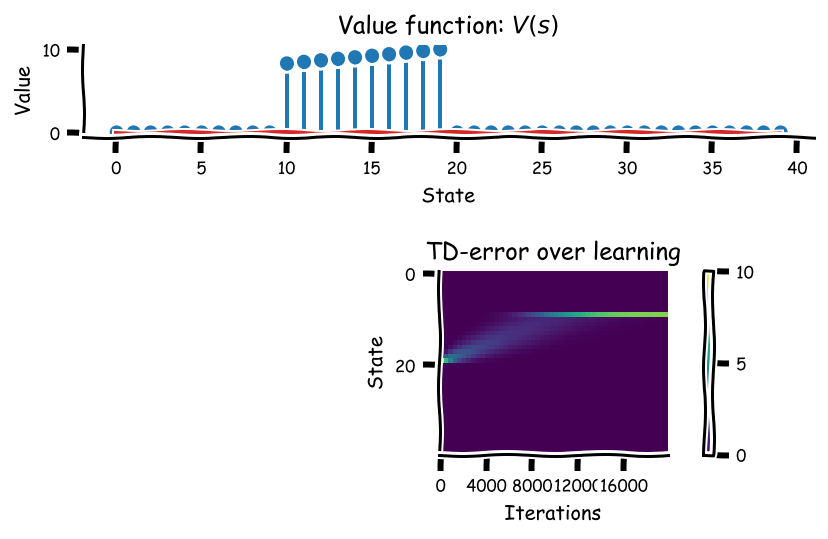
\includegraphics[scale=0.18]{Figures/RL/RL_Figure1.png}
\end{center}

\end{subbox}
\begin{subbox}{subbox}{US to CS Transfer }
\scriptsize

During classical conditioning, the subject's behavioral response (e.g., salivating) transfers from the unconditioned stimulus (US; like the smell of tasty food) to the conditioned stimulus (CS; like Pavlov ringing his bell) that predicts it. Reward prediction errors play an important role in this process by adjusting the value of states according to their expected, discounted return.

Use the widget below to examine how reward prediction errors change over time. 


Before training (orange line), only the reward state has high reward prediction error. As training progresses (blue line, slider), the reward prediction errors shift to the conditioned stimulus, where they end up when the trial is complete (green line). 

Dopamine neurons, which are thought to carry reward prediction errors \textit{in vivo}, show exactly the same behavior!
\begin{center}
    
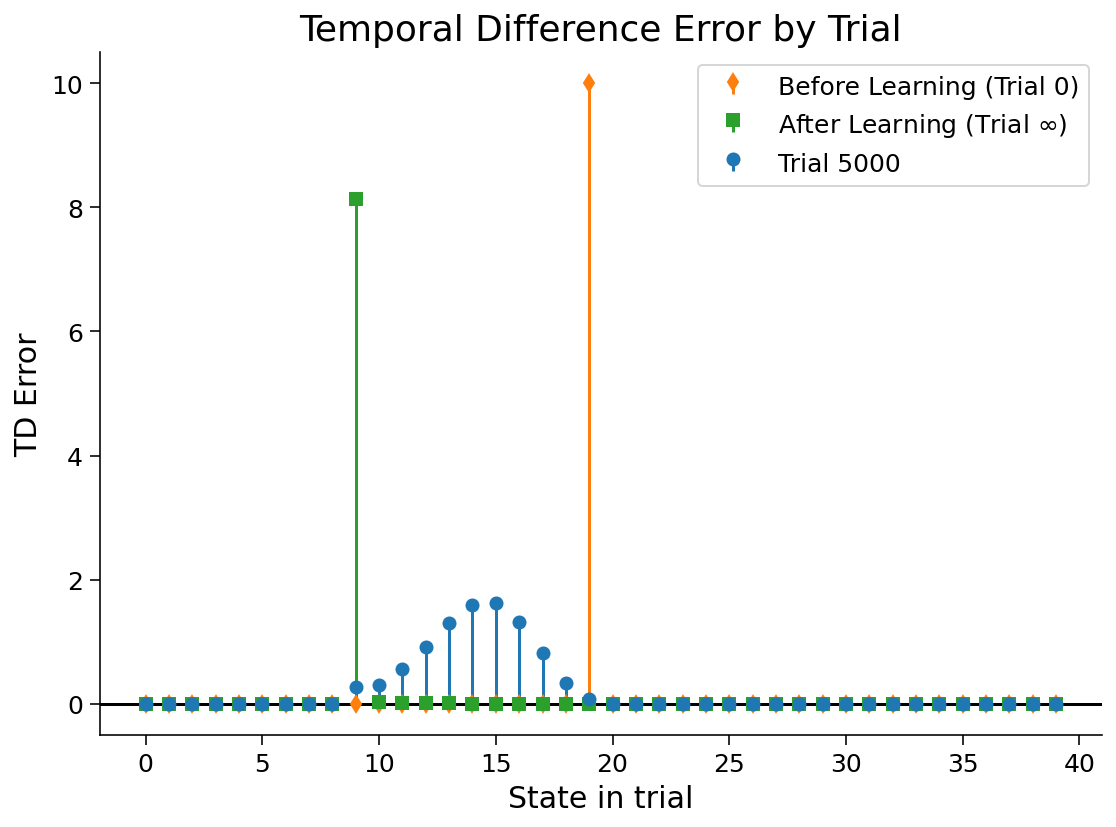
\includegraphics[scale=0.15]{Figures/RL/RL_Figure2.png}
\end{center}

\end{subbox}
\end{textbox}
%%%%%%%%%%%%%%%%%%%%%%%%%%%%%%%%%%%%%%%%%%%%%%%%%%%%%%
%%%%%%%%%%%%%%%%%%%%%%%%%%%%%%%%%%%%%%%%%%%%%%%%%%%%%%
\begin{textbox}{\href{https://compneuro.neuromatch.io/tutorials/W3D4_ReinforcementLearning/student/W3D4_Tutorial1.html}{Learning to Predict } }
\begin{subbox}{subbox}{Learning Rates and Discount Factors}
\scriptsize


Our TD-learning agent has two parameters that control how it learns: $\alpha$, the learning rate, and $\gamma$, the discount factor. In Exercise 1, we set these parameters to $\alpha=0.001$ and $\gamma=0.98$ for you. Here, you'll investigate how changing these parameters alters the model that TD-learning learns.

Before enabling the interactive demo below, take a moment to think about the functions of these two parameters. $\alpha$ controls the size of the Value function updates produced by each TD-error. In our simple, deterministic world, will this affect the final model we learn? Is a larger $\alpha$ necessarily better in more complex, realistic environments?

The discount rate $\gamma$ applies an exponentially-decaying weight to returns occuring in the future, rather than the present timestep. How does this affect the model we learn? What happens when $\gamma=0$ or $\gamma \geq 1$?

Use the widget to test your hypotheses.

\begin{center}
    
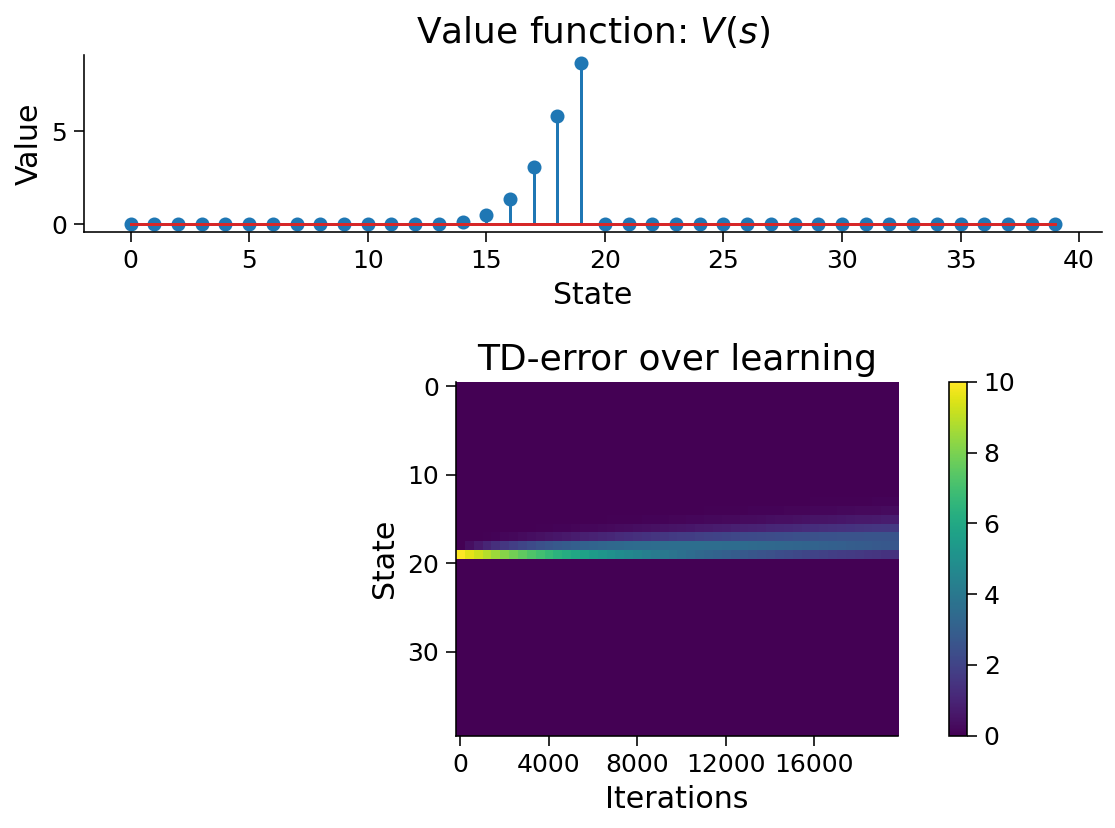
\includegraphics[scale=0.3]{Figures/RL/RL_Figure3.png}
\end{center}
$\alpha$ determines how fast the model learns. In the simple, deterministic world
we're using here, this allows the model to quickly converge onto the "true"
model that heavily values the conditioned stimulus. In more complex environments,
however, excessively large values of alpha can slow, or even prevent, learning,
as we'll see later.
$\gamma$ effectively controls how much the model cares about the future: larger values of
$\gamma$ cause the model to weigh future rewards nearly as much as present ones. At $\gamma$=1,
the model weights all rewards, regardless of when they occur, equally and when greater than one, it
starts to prefer rewards in the future, rather than the present (this is rarely good).
When $\gamma$=0, however, the model becomes greedy and only considers rewards that
can be obtained immediately.

\end{subbox}



\end{textbox}
%%%%%%%%%%%%%%%%%%%%%%%%%%%%%%%%%%%%%%%%%%%%%%%%%%%%%%
%%%%%%%%%%%%%%%%%%%%%%%%%%%%%%%%%%%%%%%%%%%%%%%%%%%%%%
\begin{textbox}{\href{https://compneuro.neuromatch.io/tutorials/W3D4_ReinforcementLearning/student/W3D4_Tutorial1.html}{Learning to Predict } }
\begin{subbox}{subbox}{TD-learning with varying reward magnitudes}
\scriptsize
In the previous exercise, the environment was as simple as possible. On every trial, the CS predicted the same reward, at the same time, with 100\% certainty. In the next few exercises, we will make the environment more progressively more complicated and examine the TD-learner's behavior.
\begin{center}
    
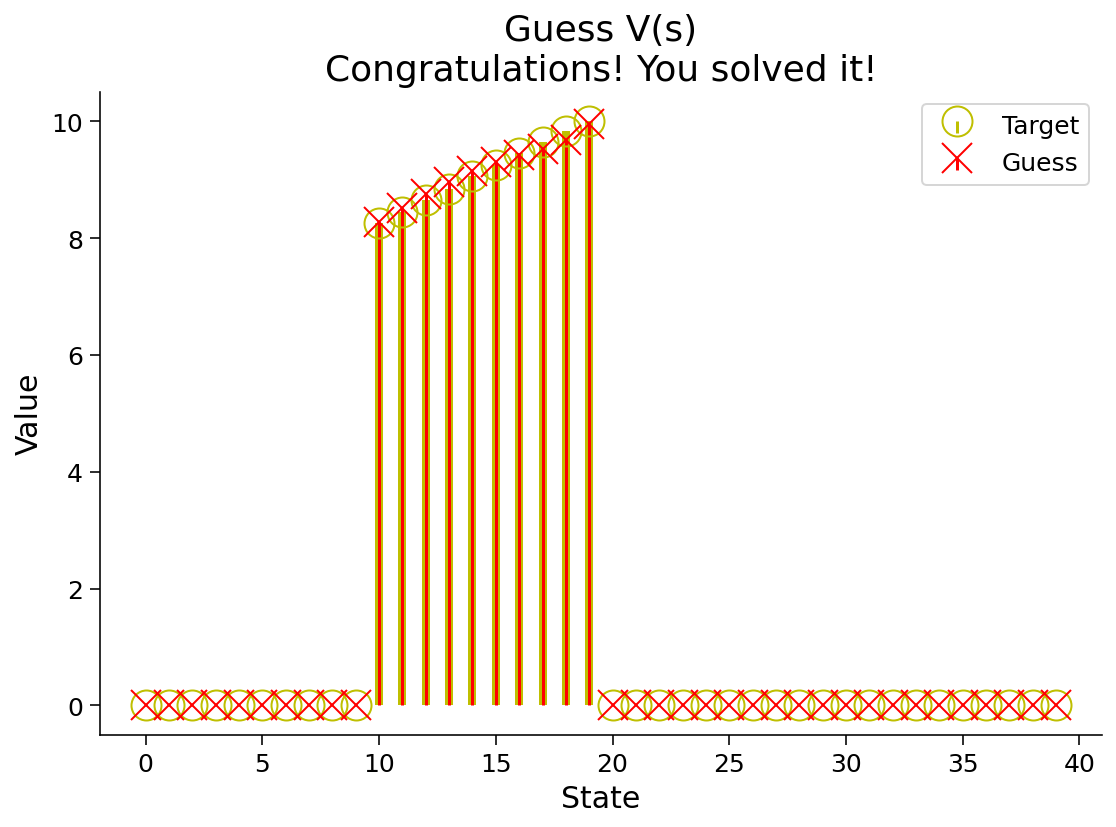
\includegraphics[scale=0.15]{Figures/RL/RL_Figure4.png}
\end{center}

\end{subbox}
\begin{subbox}{subbox}{Examining the TD Error}
\scriptsize
The plot below shows the TD errors from our multi-reward environment. A new feature appears in this plot? What is it? Why does it happen?
\begin{center}
    
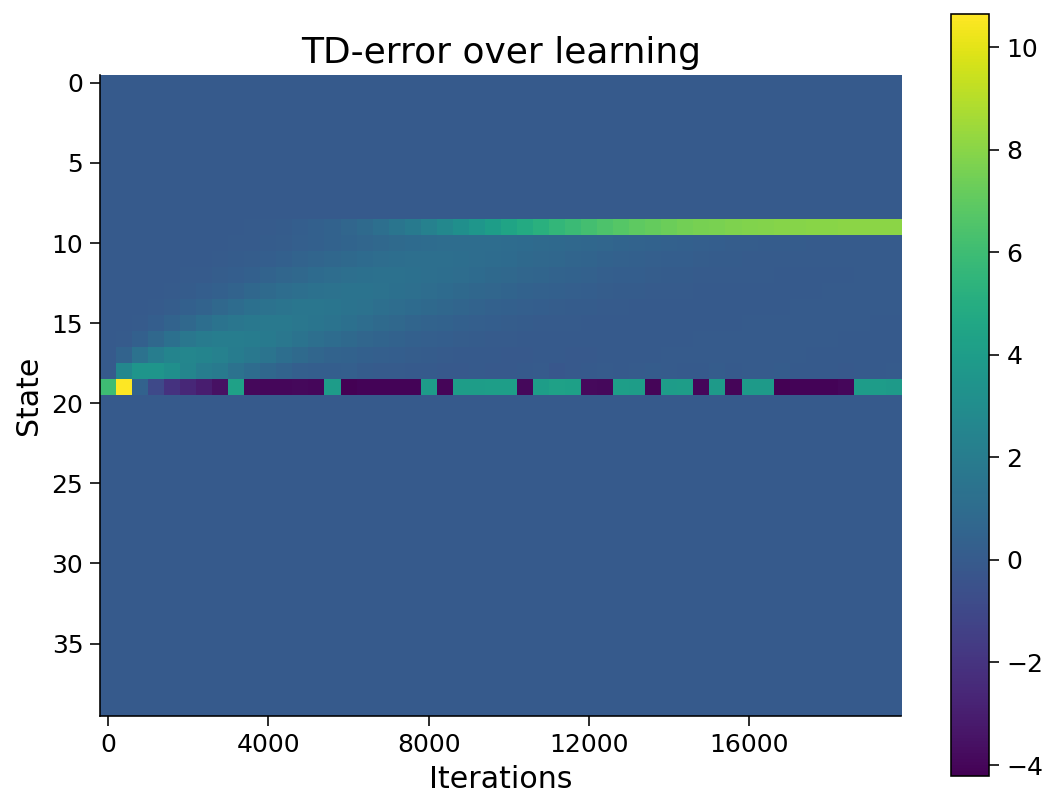
\includegraphics[scale=0.15]{Figures/RL/RL_Figure5.png}
\end{center}

\end{subbox}


\begin{subbox}{subbox}{TD-learning with probabilistic rewards}
\scriptsize
In this environment, we'll return to delivering a single reward of ten units. However, it will be delivered intermittently: on 20 percent of trials, the CS will be shown but the agent will not receive the usual reward; the remaining 80\% will proceed as usual.

 Run the cell below to simulate. How does this compare with the previous experiment?

Earlier in the notebook, we saw that changing $\alpha$ had little effect on learning in a deterministic environment. What happens if you set it to a large value, like 1, in this noisier scenario? Does it seem like it will \textit{ever} converge?
\begin{center}
    
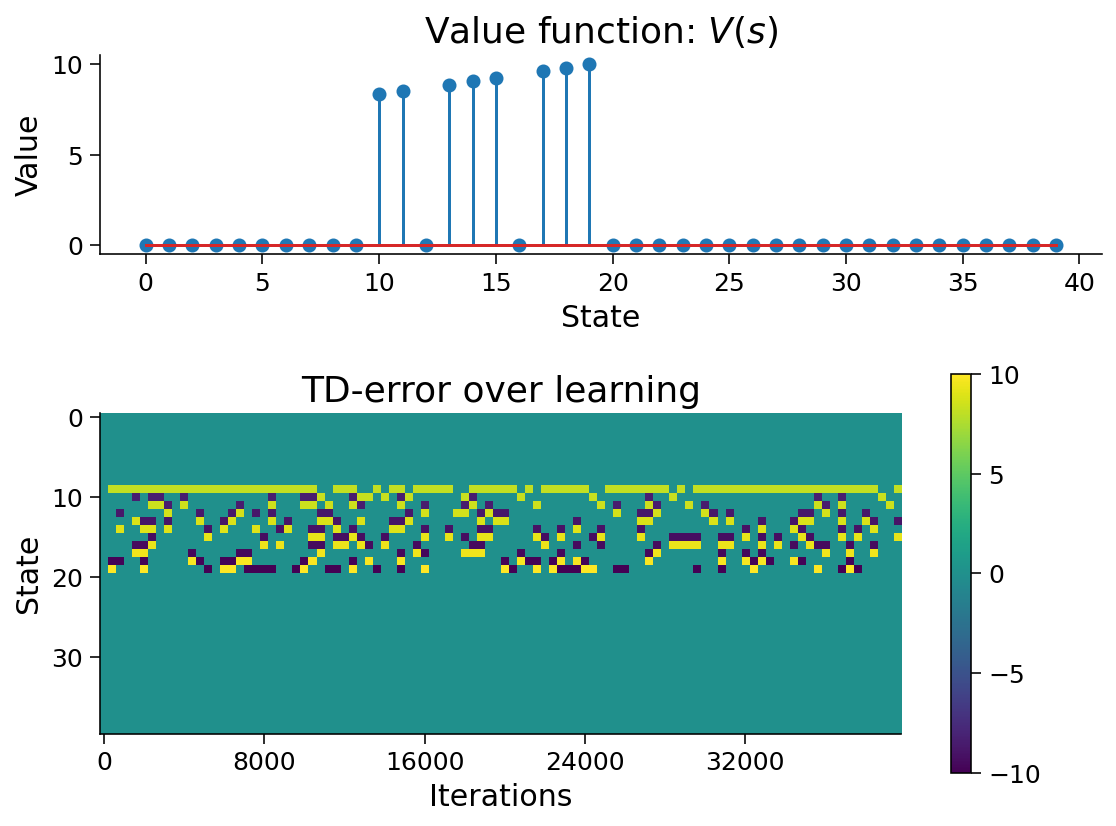
\includegraphics[scale=0.2]{Figures/RL/RL_Figure6.png}
\end{center}

\end{subbox}
\end{textbox}
%%%%%%%%%%%%%%%%%%%%%%%%%%%%%%%%%%%%%%%%%%%%%%%%%%%%%%
%%%%%%%%%%%%%%%%%%%%%%%%%%%%%%%%%%%%%%%%%%%%%%%%%%%%%%
\begin{textbox}{\href{https://compneuro.neuromatch.io/tutorials/W3D4_ReinforcementLearning/student/W3D4_Tutorial1.html}{Learning to Predict } }
\begin{subbox}{subbox}{Summary}
\scriptsize
Here, we have developed a simple TD Learner and examined how its state representations and reward prediction errors evolve during training. By manipulating its environment and parameters ($\alpha$, $\gamma$), you developed an intuition for how it behaves. 

This simple model closely resembles the behavior of subjects undergoing classical conditioning tasks and the dopamine neurons that may underlie that behavior. You may have implemented TD-reset or used the model to recreate a common experimental error. The update rule used here has been extensively studied for \href{https://www.pnas.org/content/108/Supplement_3/15647}{more than 70 years} as a possible explanation for artificial and biological learning. 

However, you may have noticed that something is missing. We carefully calculated the value of each state, but did not use it to actually do anything. Using values to plan \textbf{Actions} is coming up next!

\end{subbox}
\end{textbox}
\newpage
%%%%%%%%%%%%%%%%%%%%%%%%%%%%%%%%%%%%%%%%%%%%%%%%%%%%%%
%%%%%%%%%%%%%%%%%%%%%%%%%%%%%%%%%%%%%%%%%%%%%%%%%%%%%%
%%%%%%%% TUTORIAL 2
%%%%%%%%%%%%%%%%%%%%%%%%%%%%%%%%%%%%%%%%%%%%%%%%%%%%%%
%%%%%%%%%%%%%%%%%%%%%%%%%%%%%%%%%%%%%%%%%%%%%%%%%%%%%%
\begin{textbox}{\href{https://compneuro.neuromatch.io/tutorials/W3D4_ReinforcementLearning/student/W3D4_Tutorial2.html}{Learning to Act: Multi-Armed Bandits } }
\begin{subbox}{subbox}{Multi-Armed Bandits}
\scriptsize
Consider the following learning problem. You are faced repeatedly with a choice among $k$ different options, or actions. After each choice you receive a reward signal in the form of a numerical value, where the larger value is the better. Your objective is to maximize the expected total reward over some time period, for example, over 1000 action selections, or time steps.

This is the original form of the k-armed bandit problem. This name derives from the colloquial name for a slot machine, the "one-armed bandit", because it has the one lever to pull, and it is often rigged to take more money than it pays out over time. The multi-armed bandit extension is to imagine, for instance, that you are faced with multiple slot machines that you can play, but only one at a time. Which machine should you play, i.e., which arm should you pull, which action should you take, at any given time to maximize your total payout.


\begin{center}
    
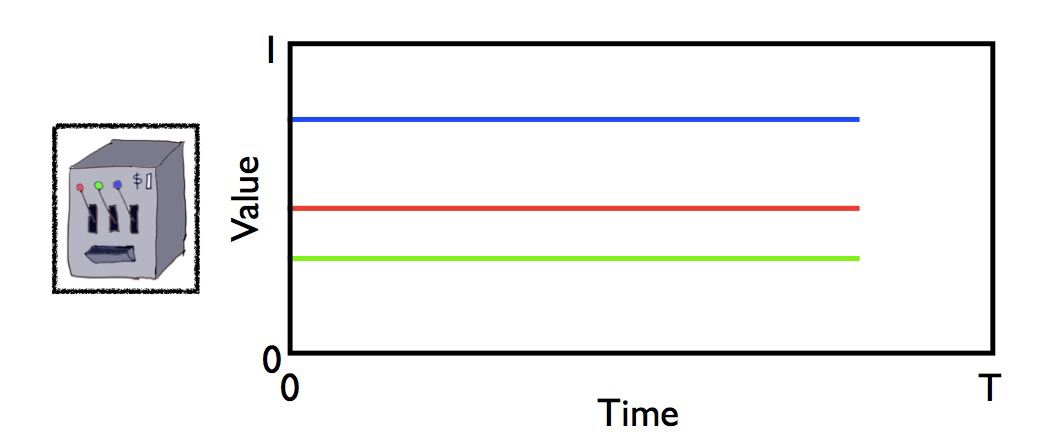
\includegraphics[scale=0.18]{Figures/RL/RL_Figure7.png}
\end{center}
While there are many different levels of sophistication and assumptions in how the rewards are determined, for simplicity's sake we will assume that each action results in a reward drawn from a fixed Gaussian distribution with unknown mean and unit variance. This problem setting is referred to as the \textit{environment}, and the goal is to find the arm with the highest mean value.

We will solve this \textit{optimization problem} with an \textit{agent}, in this case an algorithm that takes in rewards and returns actions.

\end{subbox}
\end{textbox}
%%%%%%%%%%%%%%%%%%%%%%%%%%%%%%%%%%%%%%%%%%%%%%%%%%%%%%
%%%%%%%%%%%%%%%%%%%%%%%%%%%%%%%%%%%%%%%%%%%%%%%%%%%%%%
\begin{textbox}{\href{https://compneuro.neuromatch.io/tutorials/W3D4_ReinforcementLearning/student/W3D4_Tutorial2.html}{Learning to Act: Multi-Armed Bandits } }
\begin{subbox}{subbox}{ Choosing an Action}
\scriptsize
The first thing our agent needs to be able to do is choose which arm to pull. The strategy for choosing actions based on our expectations is called a *policy* (often denoted $\pi$). We could have a random policy -- just pick an arm at random each time -- though this doesn't seem likely to be capable of optimizing our reward. We want some intentionality, and to do that we need a way of describing our beliefs about the arms' reward potential. We do this with an action-value function

\begin{equation}
q(a) = \mathbb{E} [r_{t} | a_{t} = a]
\end{equation}

where the value $q$ for taking action $a \in A$ at time $t$ is equal to the expected value of the reward $r_t$ given that we took action $a$ at that time. In practice, this is often represented as an array of values, where each action's value is a different element in the array.

Great, now that we have a way to describe our beliefs about the values each action should return, let's come up with a policy.

An obvious choice would be to take the action with the highest expected value. This is referred to as the \textit{greedy} policy

\begin{equation}
a_{t} = \text{argmax}_{a} \; q_{t} (a)
\end{equation}

where our choice action is the one that maximizes the current value function.

So far so good, but it can't be this easy. And, in fact, the greedy policy does have a fatal flaw: it easily gets trapped in local maxima. It never explores to see what it hasn't seen before if one option is already better than the others. This leads us to a fundamental challenge in coming up with effective policies.

\end{subbox}

\end{textbox}
%%%%%%%%%%%%%%%%%%%%%%%%%%%%%%%%%%%%%%%%%%%%%%%%%%%%%%
%%%%%%%%%%%%%%%%%%%%%%%%%%%%%%%%%%%%%%%%%%%%%%%%%%%%%%
\begin{textbox}{\href{https://compneuro.neuromatch.io/tutorials/W3D4_ReinforcementLearning/student/W3D4_Tutorial2.html}{Learning to Act: Multi-Armed Bandits } }

\begin{subbox}{subbox}{The Exploitation-Exploration Dilemma}
\scriptsize
If we never try anything new, if we always stick to the safe bet, we don't know what we are missing. Sometimes we aren't missing much of anything, and regret not sticking with our preferred choice, yet other times we stumble upon something new that was way better than we thought.

This is the exploitation-exploration dilemma: do you go with your best choice now, or risk the less certain option with the hope of finding something better. Too much exploration, however, means you may end up with a sub-optimal reward once it's time to stop.

In order to avoid getting stuck in local minima while also maximizing reward, effective policies need some way to balance between these two aims.

A simple extension to our greedy policy is to add some randomness. For instance, a coin flip -- heads we take the best choice now, tails we pick one at random. This is referred to as the $\epsilon$-greedy policy:

\begin{equation}
P (a_{t} = a) = 
        \begin{cases}
        1 - \epsilon + \epsilon/N    & \quad \text{if } a_{t} = \text{argmax}_{a} \; q_{t} (a) \\
        \epsilon/N        & \quad \text{else} 
        \end{cases} 
\end{equation}

which is to say that with probability 1 - $\epsilon$ for $\epsilon \in [0,1]$ we select the greedy choice, and otherwise we select an action at random (including the greedy option).

Despite its relative simplicity, the epsilon-greedy policy is quite effective, which leads to its general popularity.

The plot below shows the epsilon-greedy algorithm for deciding which action to take from a set of possible actions given their value function and a probability $\epsilon$ of simply choosing one at random. 
\begin{center}
    
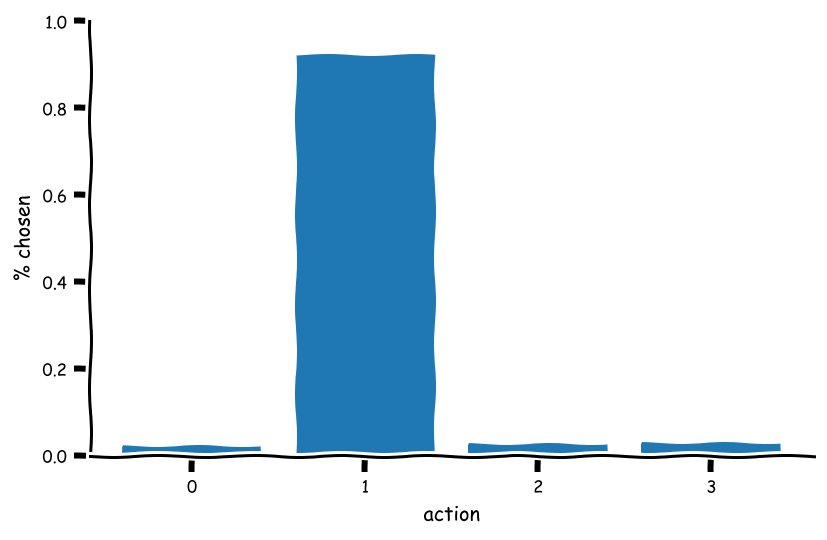
\includegraphics[scale=0.18]{Figures/RL/RL_Figure8.png}
\end{center}
This is what we should expect, that the action with the largest value (action 1) is selected about (1-$\epsilon$) of the time, or 90\% for $\epsilon = 0.1$, and the remaining 10\% is split evenly amongst the other options. Use the demo below to explore how changing $\epsilon$ affects the distribution of selected actions.

\end{subbox}
\end{textbox}
%%%%%%%%%%%%%%%%%%%%%%%%%%%%%%%%%%%%%%%%%%%%%%%%%%%%%%
%%%%%%%%%%%%%%%%%%%%%%%%%%%%%%%%%%%%%%%%%%%%%%%%%%%%%%
\begin{textbox}{\href{https://compneuro.neuromatch.io/tutorials/W3D4_ReinforcementLearning/student/W3D4_Tutorial2.html}{Learning to Act: Multi-Armed Bandits } }

\begin{subbox}{subbox}{Solving Multi-Armed Bandits}
\scriptsize

Now that we have both a policy and a learning rule, we can combine these to solve our original multi-armed bandit task. Recall that we have some number of arms that give rewards drawn from Gaussian distributions with unknown mean and unit variance, and our goal is to find the arm with the highest mean.

We can use our multi-armed bandit method to evaluate how our epsilon-greedy policy and learning rule perform at solving the task. First we will set our environment to have 10 arms and our agent parameters to $\epsilon=0.1$ and $\alpha=0.01$. In order to get a good sense of the agent's performance, we will run the episode for 1000 steps.
\begin{center}
    
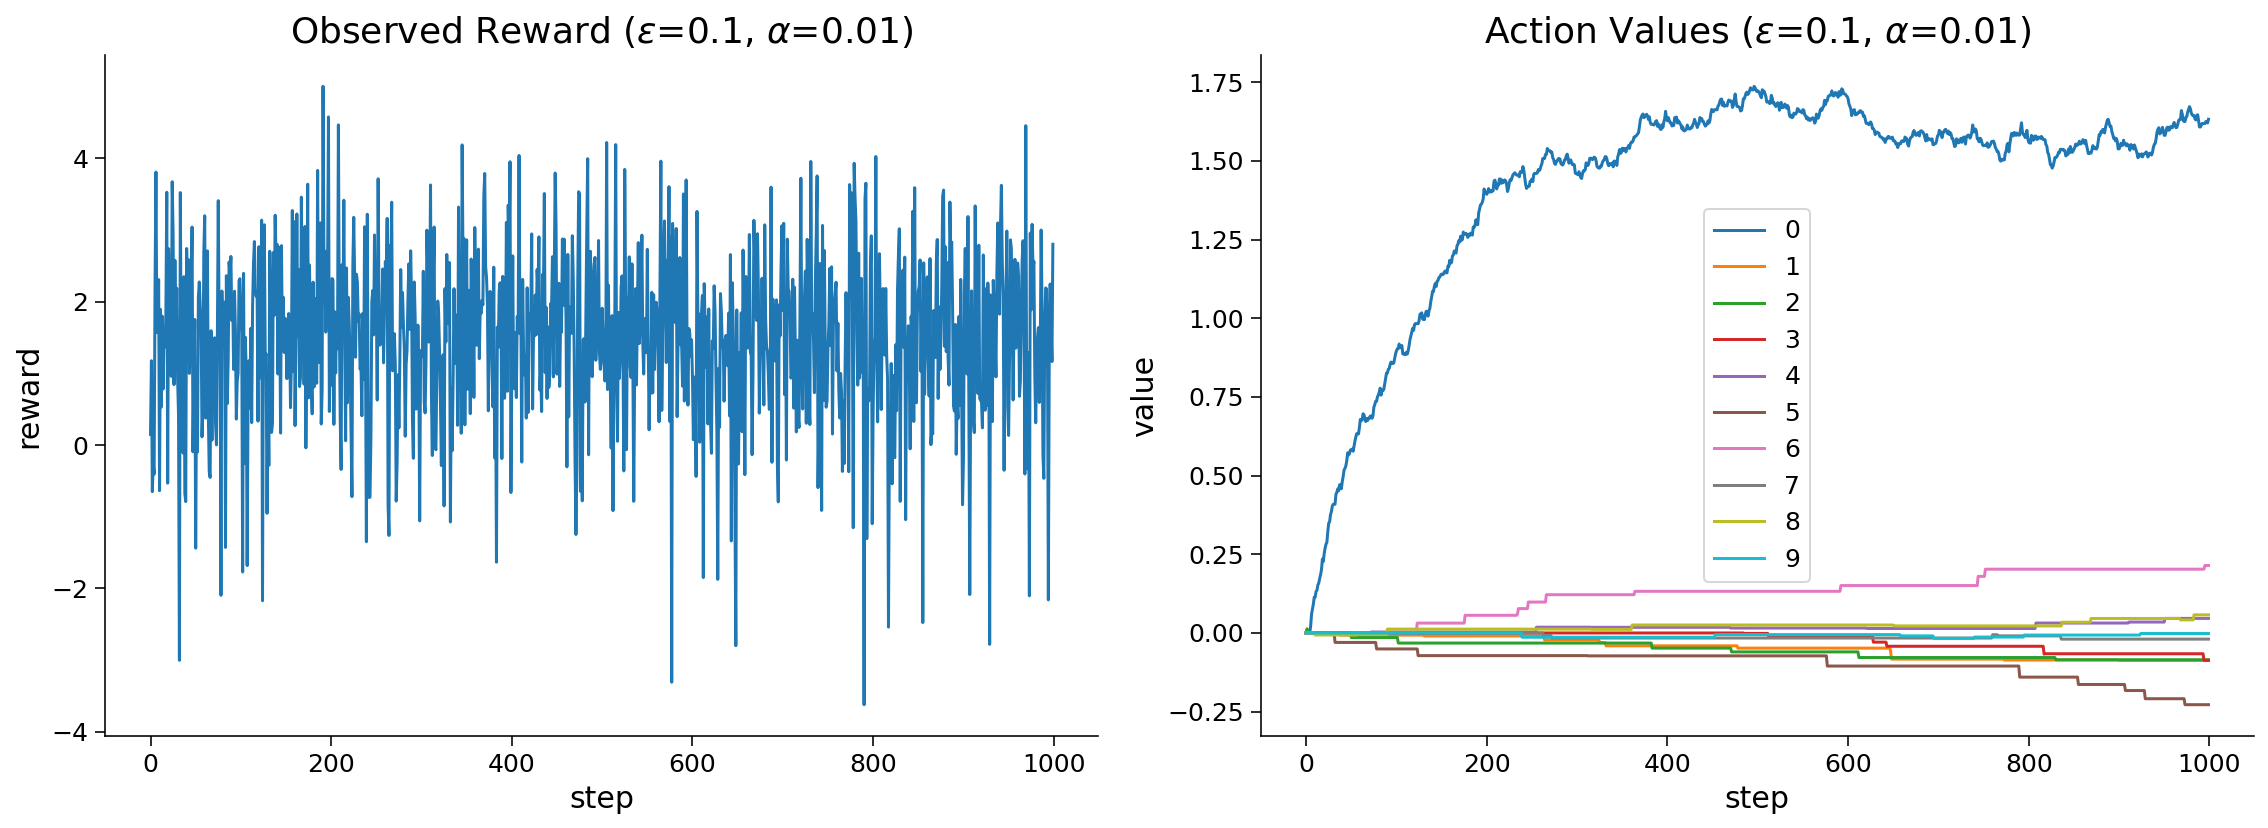
\includegraphics[scale=0.15]{Figures/RL/RL_Figure9.png}
\end{center}

Alright, we got some rewards that are kind of all over the place, but the agent seemed to settle in on the first arm as the preferred choice of action relatively quickly. Let's see how well we did at recovering the true means of the Gaussian random variables behind the arms.
\begin{center}
    
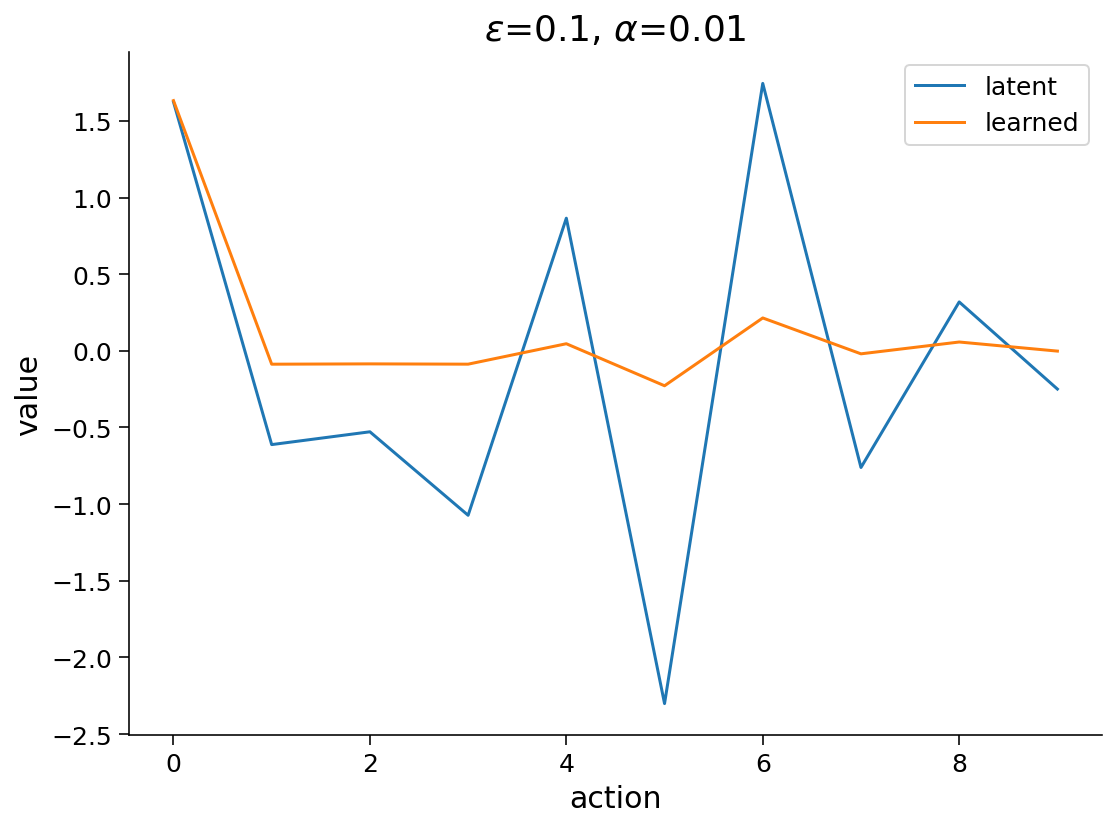
\includegraphics[scale=0.15]{Figures/RL/RL_Figure10.png}
\end{center}


Well, we seem to have found a very good estimate for action 0, but most of the others are not great. In fact, we can see the effect of the local maxima trap at work -- the greedy part of our algorithm locked onto action 0, which is actually the 2nd best choice to action 6. Since these are the means of Gaussian random variables, we can see that the overlap between the two would be quite high, so even if we did explore action 6, we may draw a sample that is still lower than our estimate for action 0.

However, this was just one choice of parameters. Perhaps there is a better combination?

\end{subbox}
\end{textbox}
%%%%%%%%%%%%%%%%%%%%%%%%%%%%%%%%%%%%%%%%%%%%%%%%%%%%%%
%%%%%%%%%%%%%%%%%%%%%%%%%%%%%%%%%%%%%%%%%%%%%%%%%%%%%%
\begin{textbox}{\href{https://compneuro.neuromatch.io/tutorials/W3D4_ReinforcementLearning/student/W3D4_Tutorial2.html}{Learning to Act: Multi-Armed Bandits } }

\begin{subbox}{subbox}{Changing Epsilon and Alpha}
\scriptsize
By varying the values of $\epsilon$ (exploitation-exploration tradeoff), $\alpha$ (learning rate), and even the number of actions $k$, changes the behavior of our agent.


\begin{center}
    
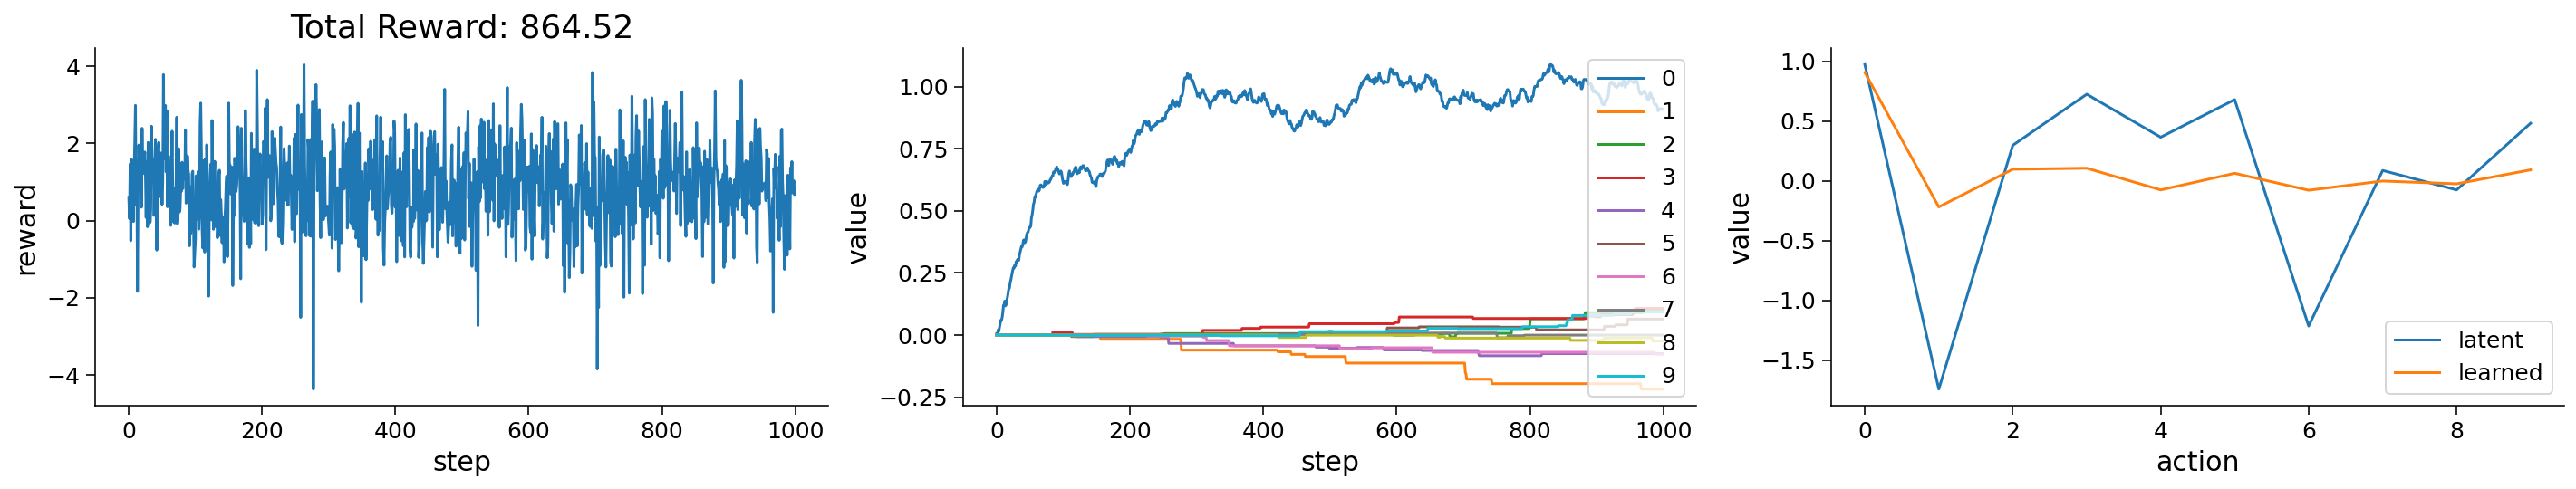
\includegraphics[scale=0.13]{Figures/RL/RL_Figure11.png}
\end{center}

While we can see how changing the $\epsilon$ and $\alpha$ values impact the agent's behavior, this doesn't give us a great sense of which combination is optimal. Due to the stochastic nature of both our rewards and our policy, a single trial run isn't sufficient to give us this information. Let's run multiple trials and compare the average performance.

First we will look at different values for $\epsilon \in [0.0, 0.1, 0.2]$ to a fixed $\alpha=0.1$. We will run 200 trials as a nice balance between speed and accuracy.

\begin{center}
    
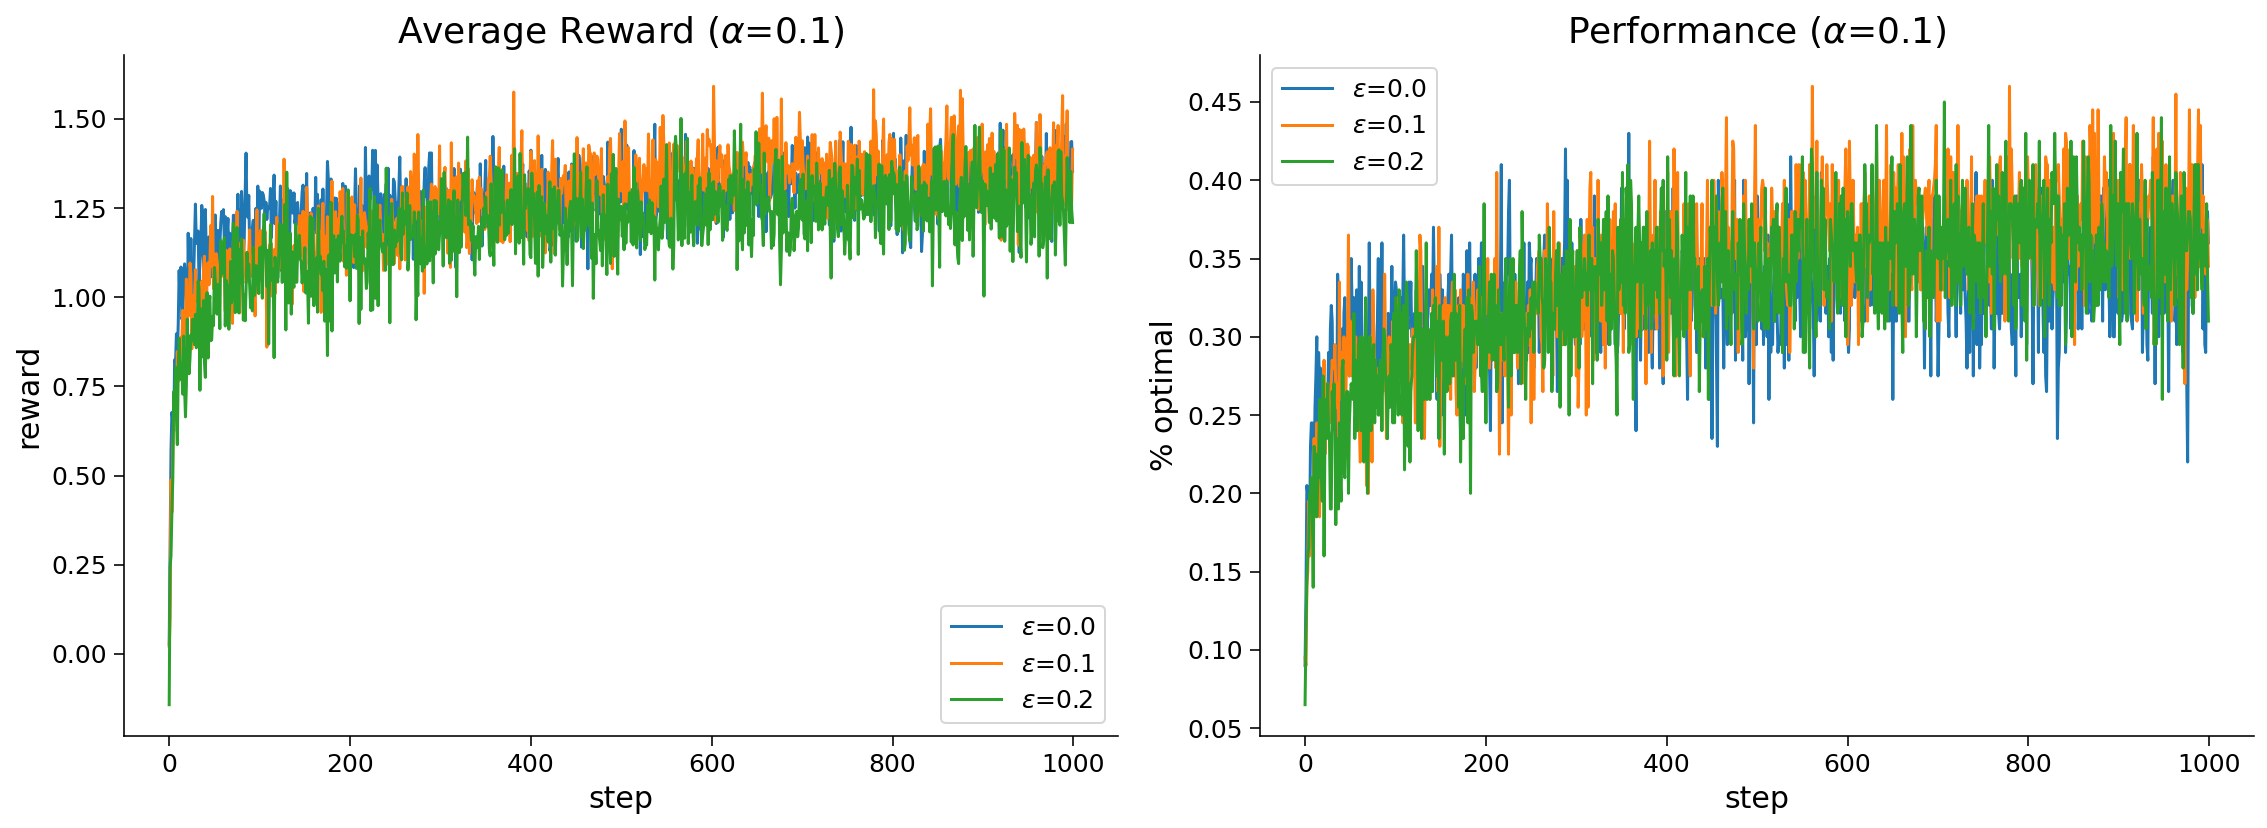
\includegraphics[scale=0.15]{Figures/RL/RL_Figure12.png}
\end{center}
On the left we have plotted the average reward over time, and we see that while $\epsilon=0$ (the greedy policy) does well initially, $\epsilon=0.1$ starts to do slightly better in the long run, while $\epsilon=0.2$ does the worst. Looking on the right, we see the percentage of times the optimal action (the best possible choice at time $t$) was taken, and here again we see a similar pattern of $\epsilon=0.1$ starting out a bit slower but eventually having a slight edge in the longer run.

We can also do the same for the learning rates. We will evaluate $\alpha \in [0.01, 0.1, 1.0]$ to a fixed $\epsilon=0.1$.

\begin{center}
    
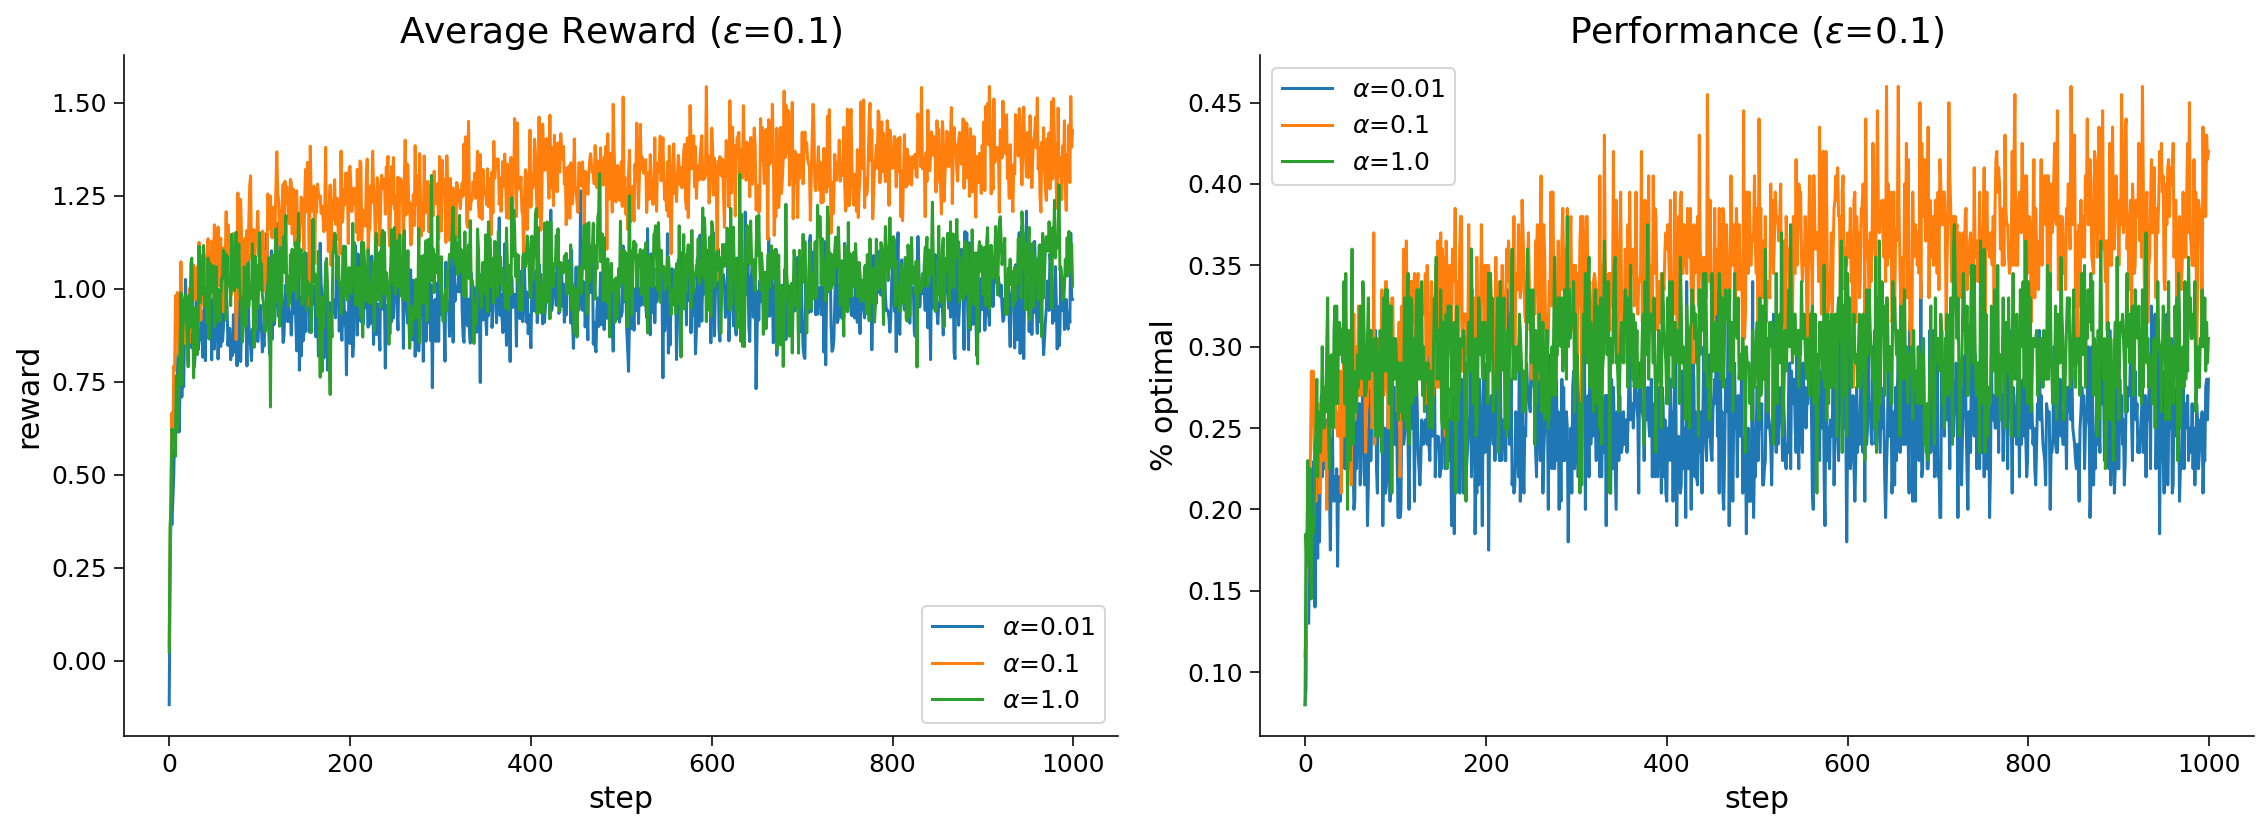
\includegraphics[scale=0.15]{Figures/RL/RL_Figure13.png}
\end{center}
Again we see a balance between an effective learning rate. $\alpha=0.01$ is too weak to quickly incorporate good values, while $\alpha=1$ is too strong likely resulting in high variance in values due to the Gaussian nature of the rewards.

\end{subbox}
\end{textbox}
\newpage
%%%%%%%%%%%%%%%%%%%%%%%%%%%%%%%%%%%%%%%%%%%%%%%%%%%%%%
%%%%%%%%%%%%%%%%%%%%%%%%%%%%%%%%%%%%%%%%%%%%%%%%%%%%%%
%%% TUTORIAL 3
%%%%%%%%%%%%%%%%%%%%%%%%%%%%%%%%%%%%%%%%%%%%%%%%%%%%%%
%%%%%%%%%%%%%%%%%%%%%%%%%%%%%%%%%%%%%%%%%%%%%%%%%%%%%%
\begin{textbox}{\href{https://compneuro.neuromatch.io/tutorials/W3D4_ReinforcementLearning/student/W3D4_Tutorial3.html}{Learning to Act: Q-Learning } }

\begin{subbox}{subbox}{Overview}
\scriptsize
Here you will learn how to act in the more realistic setting of sequential decisions, formalized by Markov Decision Processes (MDPs). In a sequential decision problem, the actions executed in one state not only may lead to immediate rewards (as in a bandit problem), but may also affect the states experienced next (unlike a bandit problem). Each individual action may therefore affect all future rewards. Thus, making decisions in this setting requires considering each action in terms of their expected \textbf{cumulative} future reward.

We will consider here the example of spatial navigation, where actions (movements) in one state (location) affect the states experienced next, and an agent might need to execute a whole sequence of actions before a reward is obtained.


\end{subbox}

\begin{subbox}{subbox}{Markov Decision Processes}
\scriptsize
\textbf{Grid Worlds}\\

As pointed out, bandits only have a single state and immediate rewards for our actions. Many problems we are interested in have multiple states and delayed rewards, i.e. we won't know if the choices we made will pay off over time, or which actions we took contributed to the outcomes we observed.

In order to explore these ideas, we turn to the common problem setting: the grid world. Grid worlds are simple environments where each state corresponds to a tile on a 2D grid, and the only actions the agent can take are to move up, down, left, or right across the grid tiles. The agent's job is almost always to find a way to a goal tile in the most direct way possible while overcoming some maze or other obstacles, either static or dynamic.

For our discussion we will be looking at the classic Cliff World, or Cliff Walker, environment. This is a $4 \times 10$ grid with a starting position in the lower-left and the goal position in the lower-right. Every tile between these two is the "cliff", and should the agent enter the cliff, they will receive a -100 reward and be sent back to the starting position. Every tile other than the cliff produces a -1 reward when entered. The goal tile ends the episode after taking any action from it.

\begin{center}
    
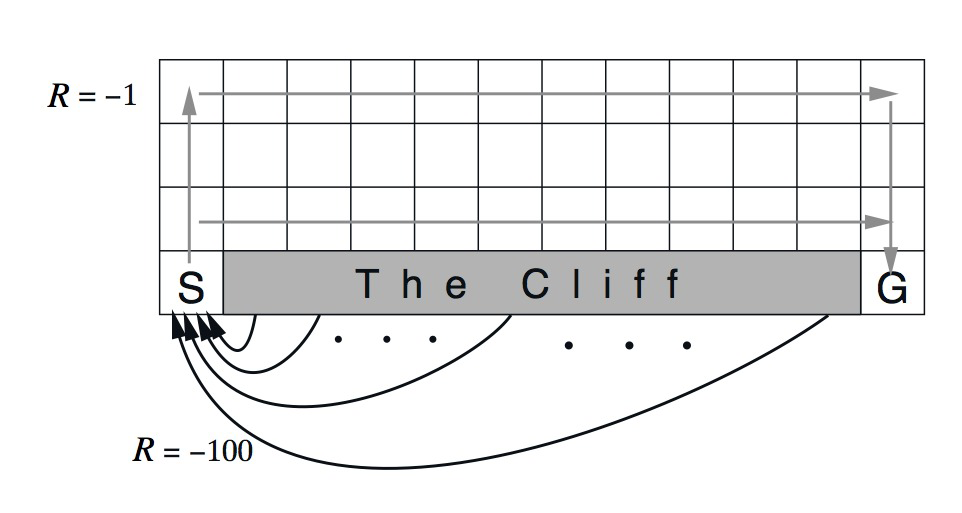
\includegraphics[scale=0.14]{Figures/RL/RL_Figure14.png}
\end{center}

Given these conditions, the maximum achievable reward is -11 (1 up, 9 right, 1 down). Using negative rewards is a common technique to encourage the agent to move and seek out the goal state as fast as possible.

\end{subbox}
\end{textbox}
%%%%%%%%%%%%%%%%%%%%%%%%%%%%%%%%%%%%%%%%%%%%%%%%%%%%%%
%%%%%%%%%%%%%%%%%%%%%%%%%%%%%%%%%%%%%%%%%%%%%%%%%%%%%%
\begin{textbox}{\href{https://compneuro.neuromatch.io/tutorials/W3D4_ReinforcementLearning/student/W3D4_Tutorial3.html}{Learning to Act: Q-Learning } }

\begin{subbox}{subbox}{Q-Learning}
\scriptsize

Now that we have our environment, how can we solve it? 

One of the most famous algorithms for estimating action values (aka Q-values) is the Temporal Differences (TD) control algorithm known as Q-learning (Watkins, 1989). 
\begin{eqnarray*}
Q(s_t,a_t) &\leftarrow& Q(s_t,a_t) + \\& & \alpha \big(r_t + \gamma\max_{\limits{a}} Q(s_{t+1},a_{t+1}) - Q(s_t,a_t)\big)
\end{eqnarray*}

where $Q(s,a)$ is the value function for action $a$ at state $s$, $\alpha$ is the learning rate, $r$ is the reward, and $\gamma$ is the temporal discount rate.

The expression $r_t + \gamma\max_{\limits{a}} Q(s_{t+1},a_{t+1})$ is referred to as the TD target while the full expression

\begin{equation}
r_t + \gamma\max_{\limits{a}} Q(s_{t+1},a_{t+1}) - Q(s_t,a_t),
\end{equation}

i.e., the difference between the TD target and the current Q-value, is referred to as the TD error, or reward prediction error.

Because of the max operator used to select the optimal Q-value in the TD target, Q-learning directly estimates the optimal action value, i.e., the cumulative future reward that would be obtained if the agent behaved optimally, regardless of the policy currently followed by the agent. For this reason, Q-learning is referred to as an \textbf{off-policy} method.


\end{subbox}

\begin{subbox}{subbox}{Implement the Q-learning algorithm}
\scriptsize



The top left is a representation of the Q-table itself, showing the values for different actions in different states. Notably, going right from the starting state or down when above the cliff is clearly very bad.\\
 The top right figure shows the greedy policy based on the Q-table, i.e. what action would the agent take if it only took its best guess in that state.\\
 The bottom right is the same as the top, only instead of showing the action, it's showing a representation of the maximum Q-value at a particular state.\\
 The bottom left is the actual proof of learning, as we see the total reward steadily increasing after each episode until asymptoting at the maximum possible reward of -11.

\begin{center}
    
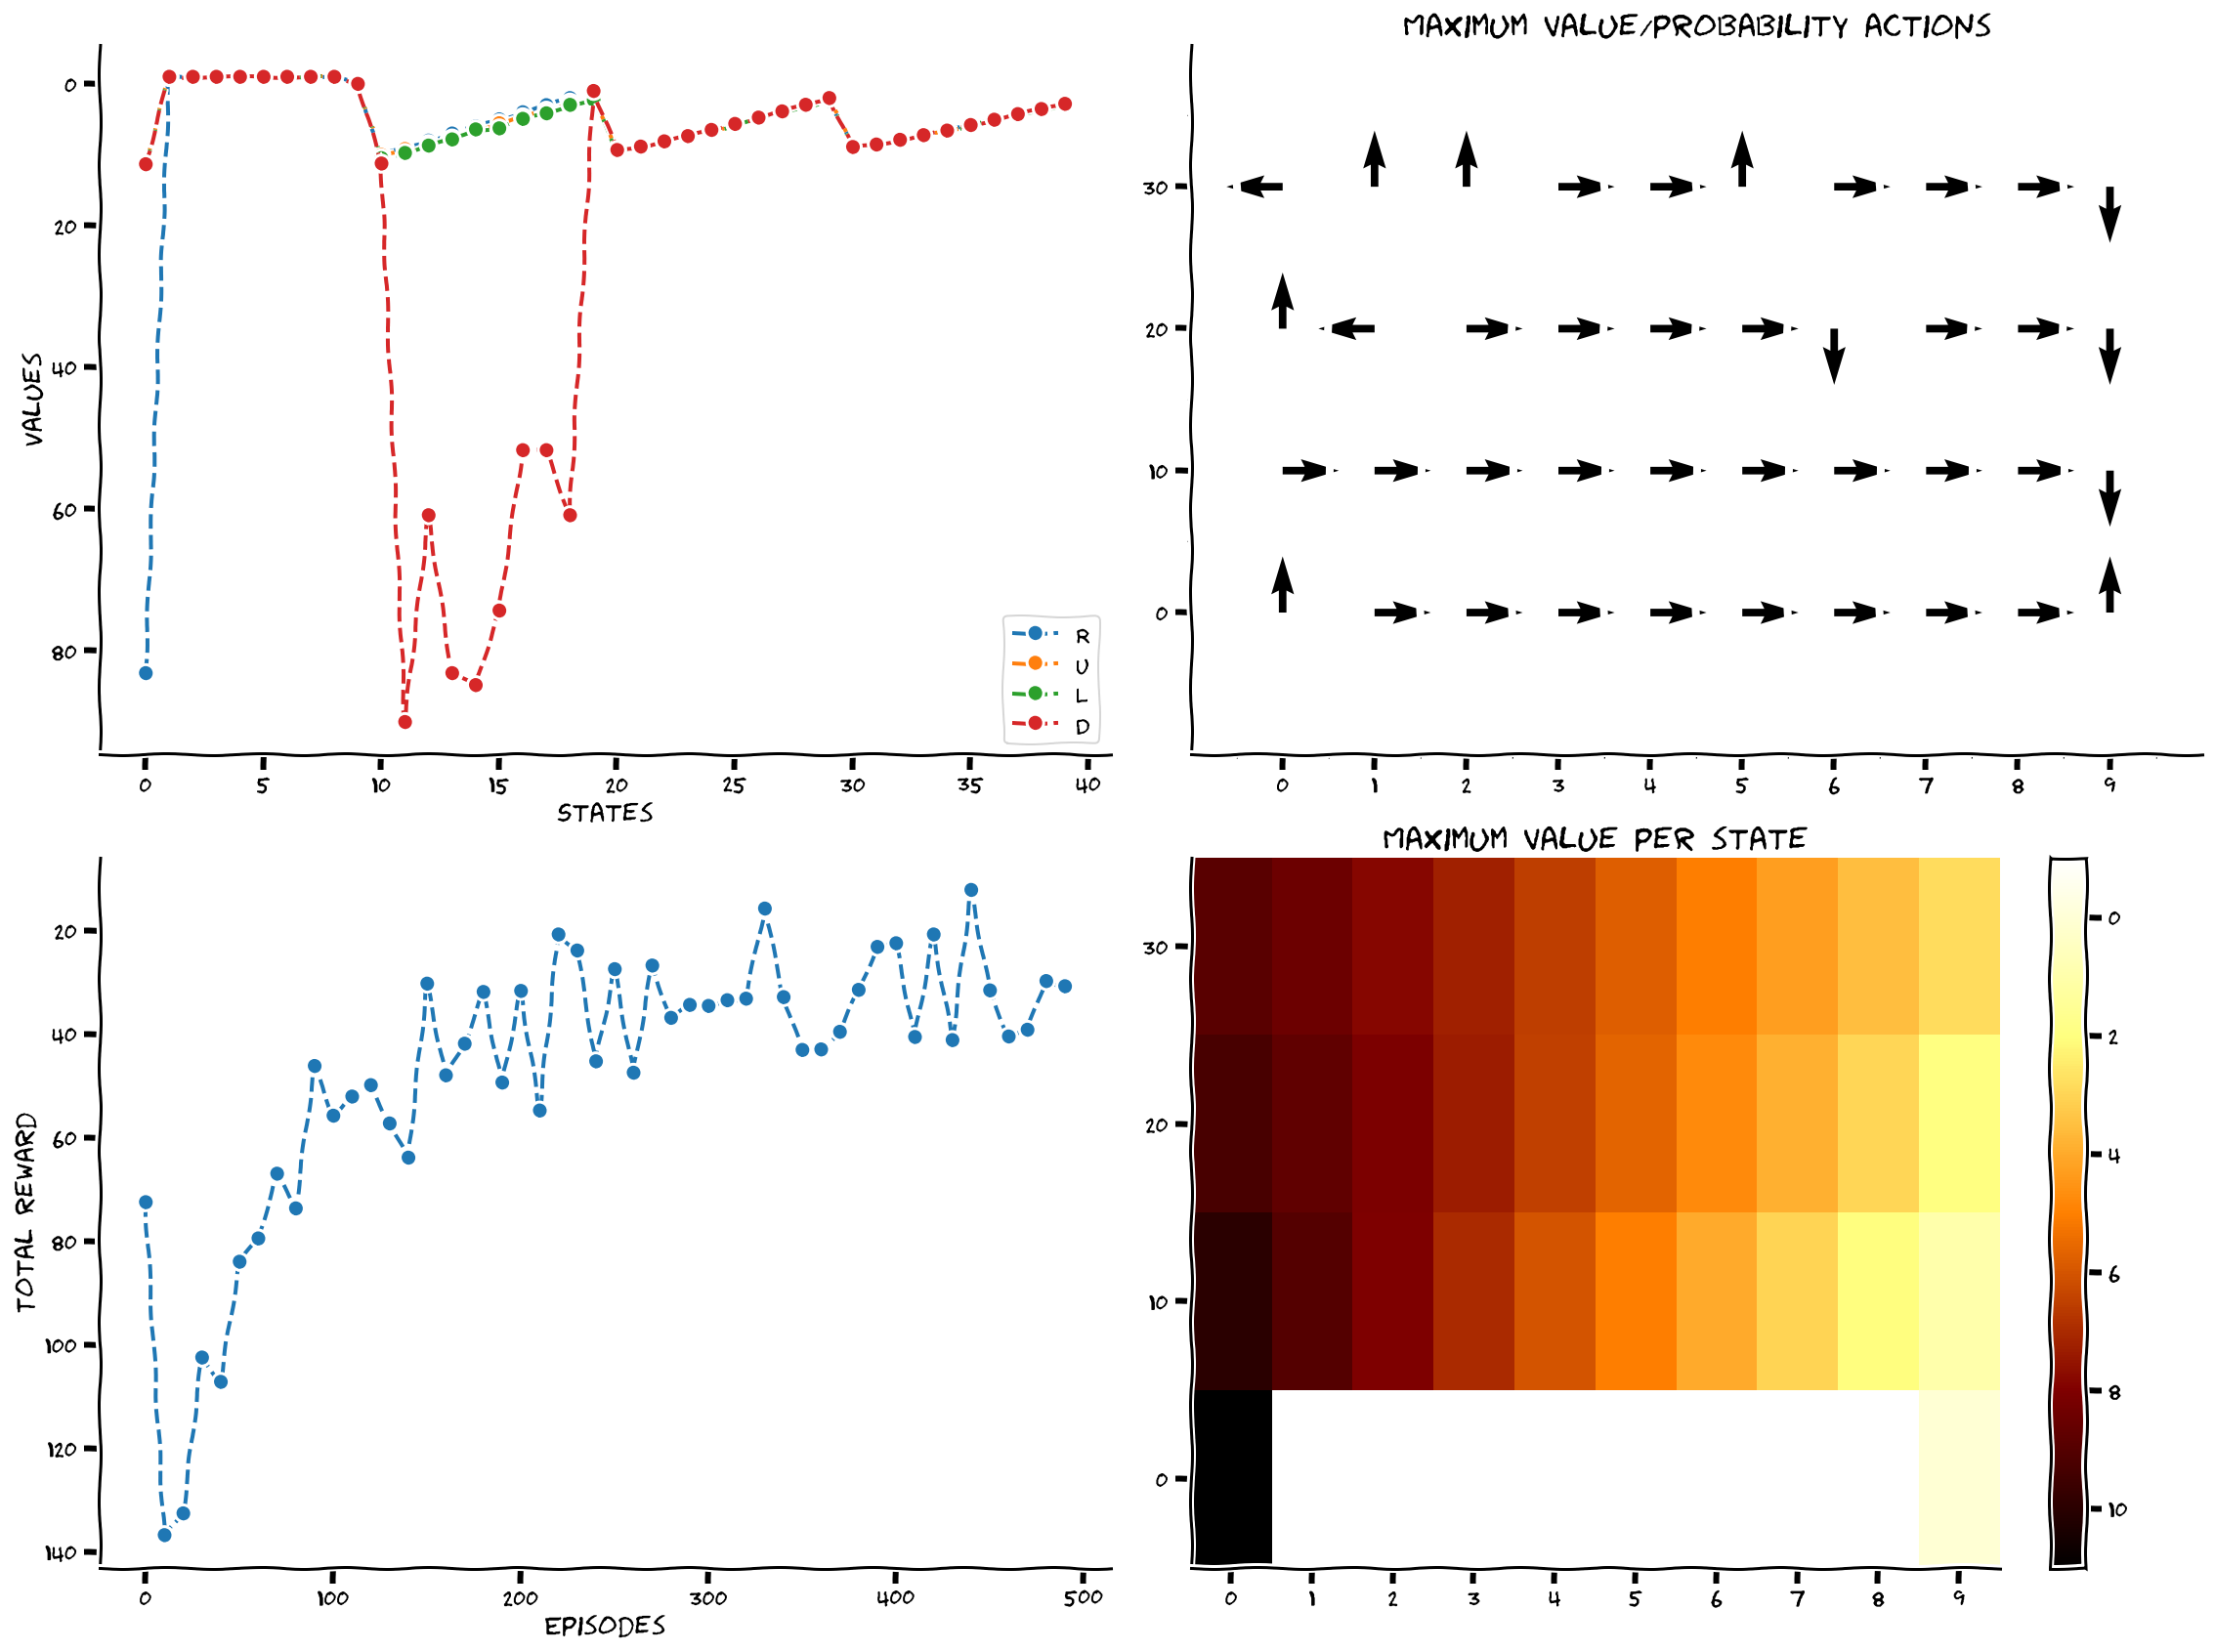
\includegraphics[scale=0.13]{Figures/RL/RL_Figure15.png}
\end{center}



\end{subbox}
\end{textbox}
\newpage
%%%%%%%%%%%%%%%%%%%%%%%%%%%%%%%%%%%%%%%%%%%%%%%%%%%%%%
%%%%%%%%%%%%%%%%%%%%%%%%%%%%%%%%%%%%%%%%%%%%%%%%%%%%%%
%%% TUTORIAL 4
%%%%%%%%%%%%%%%%%%%%%%%%%%%%%%%%%%%%%%%%%%%%%%%%%%%%%%
%%%%%%%%%%%%%%%%%%%%%%%%%%%%%%%%%%%%%%%%%%%%%%%%%%%%%%
\begin{textbox}{\href{https://compneuro.neuromatch.io/tutorials/W3D4_ReinforcementLearning/student/W3D4_Tutorial4.html}{From Reinforcement Learning to Planning } }

\begin{subbox}{subbox}{Model-based RL}
\scriptsize
The algorithms introduced in the previous tutorials are all *model-free*, as they do not require a model to use or control behavior. In this section, we will study a different class of algorithms called model-based. As we will see next, in contrast to model-free RL, model-based methods use a model to build a policy.

But what is a model? A model (sometimes called a world model or internal model) is a representation of how the world will respond to the agent's actions. You can think of it as a representation of how the world \textit{works}. With such a representation, the agent can simulate new experiences and learn from these simulations. This is advantageous for two reasons. First, acting in the real world can be costly and sometimes even dangerous. Learning from simulated experience can avoid some of these costs or risks. Second, simulations make fuller use of one's limited experience. To see why, imagine an agent interacting with the real world. The information acquired with each individual action can only be assimilated at the moment of the interaction. In contrast, the experiences simulated from a model can be simulated multiple times -- and whenever desired -- allowing for the information to be more fully assimilated.

Our RL agent will act in the Quentin's world, a 10x10 grid world. 
\begin{center}
    
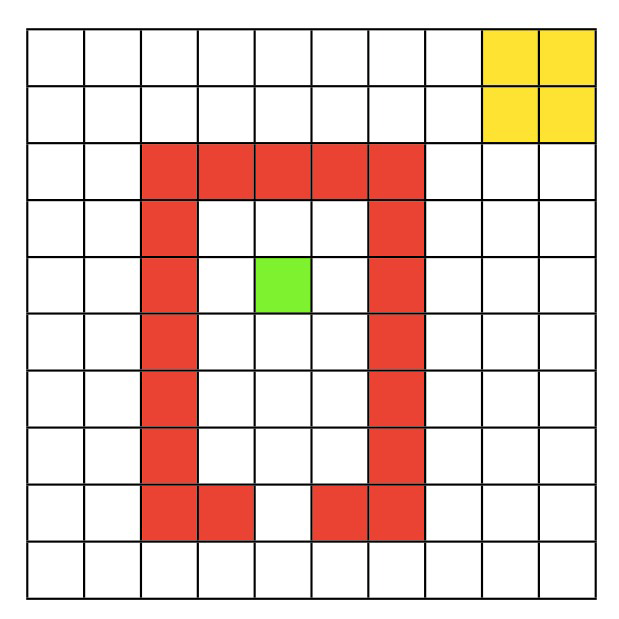
\includegraphics[scale=0.14]{Figures/RL/RL_Figure16.png}
\end{center}
In this environment, there are 100 states and 4 possible actions: right, up, left, and down. The goal of the agent is to move, via a series of steps, from the start (green) location to the goal (yellow) region, while avoiding the red walls. More specifically:
\begin{itemize}
    \item 
 The agent starts in the green state,
\item Moving into one of the red states incurs a reward of -1,
\item Moving into the world borders stays in the same place,
\item Moving into the goal state (yellow square in the upper right corner) gives you a reward of 1, and
\item Moving anywhere from the goal state ends the episode.
\end{itemize}

Now that we have our environment and task defined, how can we solve this using a model-based RL agent?

\end{subbox}

\end{textbox}
%%%%%%%%%%%%%%%%%%%%%%%%%%%%%%%%%%%%%%%%%%%%%%%%%%%%%%
%%%%%%%%%%%%%%%%%%%%%%%%%%%%%%%%%%%%%%%%%%%%%%%%%%%%%%
\begin{textbox}{\href{https://compneuro.neuromatch.io/tutorials/W3D4_ReinforcementLearning/student/W3D4_Tutorial4.html}{From Reinforcement Learning to Planning } }

\begin{subbox}{subbox}{ Dyna-Q}
\scriptsize
In this section, we will implement Dyna-Q, one of the simplest model-based reinforcement learning algorithms. A Dyna-Q agent combines acting, learning, and planning. The first two components -- acting and learning -- are just like what we have studied previously. Q-learning, for example, learns by acting in the world, and therefore combines acting and learning. But a Dyna-Q agent also implements planning, or simulating experiences from a model--and learns from them. 

In theory, one can think of a Dyna-Q agent as implementing acting, learning, and planning simultaneously, at all times. But, in practice, one needs to specify the algorithm as a sequence of steps. The most common way in which the Dyna-Q agent is implemented is by adding a planning routine to a Q-learning agent: after the agent acts in the real world and learns from the observed experience, the agent is allowed a series of $k$ *planning steps*. At each one of those $k$ planning steps, the model generates a simulated experience by randomly sampling from the history of all previously experienced state-action pairs. The agent then learns from this simulated experience, again using the same Q-learning rule that you implemented for learning from real experience. This simulated experience is simply a one-step transition, i.e., a state, an action, and the resulting state and reward. So, in practice, a Dyna-Q agent learns (via Q-learning) from one step of \textbf{real} experience during acting, and then from k steps of \textbf{simulated} experience during planning.

There's one final detail about this algorithm: where does the simulated experiences come from or, in other words, what is the "model"? In Dyna-Q, as the agent interacts with the environment, the agent also learns the model. For simplicity, Dyna-Q implements model-learning in an almost trivial way, as simply caching the results of each transition. Thus, after each one-step transition in the environment, the agent saves the results of this transition in a big matrix, and consults that matrix during each of the planning steps. Obviously, this model-learning strategy only makes sense if the world is deterministic (so that each state-action pair always leads to the same state and reward), and this is the setting of the exercise below. However, even this simple setting can already highlight one of Dyna-Q major strengths: the fact that the planning is done at the same time as the agent interacts with the environment, which means that new information gained from the interaction may change the model and thereby interact with planning in potentially interesting ways.

\end{subbox}
\end{textbox}
%%%%%%%%%%%%%%%%%%%%%%%%%%%%%%%%%%%%%%%%%%%%%%%%%%%%%%
%%%%%%%%%%%%%%%%%%%%%%%%%%%%%%%%%%%%%%%%%%%%%%%%%%%%%%
\begin{textbox}{\href{https://compneuro.neuromatch.io/tutorials/W3D4_ReinforcementLearning/student/W3D4_Tutorial4.html}{From Reinforcement Learning to Planning } }

\begin{subbox}{subbox}{Dyna-Q Algorithm}
\scriptsize

Initialize $Q(s,a)$ and $Model(s,a)$ for all $s \in S$ and $a \in A$.\\
Loop forever:\\
\begin{enumerate}[label=(\alph*)]
    \item 
 $S$ $\leftarrow$ current (nonterminal) state 
 \item  $A$ $\leftarrow$ $\epsilon$-greedy$(S,Q)$ 
   \item  Take action $A$; observe resultant reward, $R$, and state, $S'$ 
   \item  $Q(S,A)\leftarrow Q(S,A) + \alpha \left[R + \gamma \max_{a} Q(S',a) - Q(S,A)\right]$ 
   \item  $Model(S,A)$ $\leftarrow$ $R,S'$ (assuming deterministic environment) 
   \item  Loop repeat $k$ times: 
 $S$ $\leftarrow$ random previously observed state \\
 $A$ $\leftarrow$ random action previously taken in $S$ \\
 $R,S'$ $\leftarrow$ $Model(S,A)$ \\
 $Q(S,A) \leftarrow Q(S,A) + \alpha \left[R + \gamma \max_{a} Q(S',a) - Q(S,A)\right]$ 
\end{enumerate}

\end{subbox}

\begin{subbox}{subbox}{Implementing Dyna-Q}
\scriptsize

The plot below show an implementation of Dyna-Q  planning to try and solve Quentin's World. Notice that we set the number of planning steps $k=10$.
\begin{center}
    
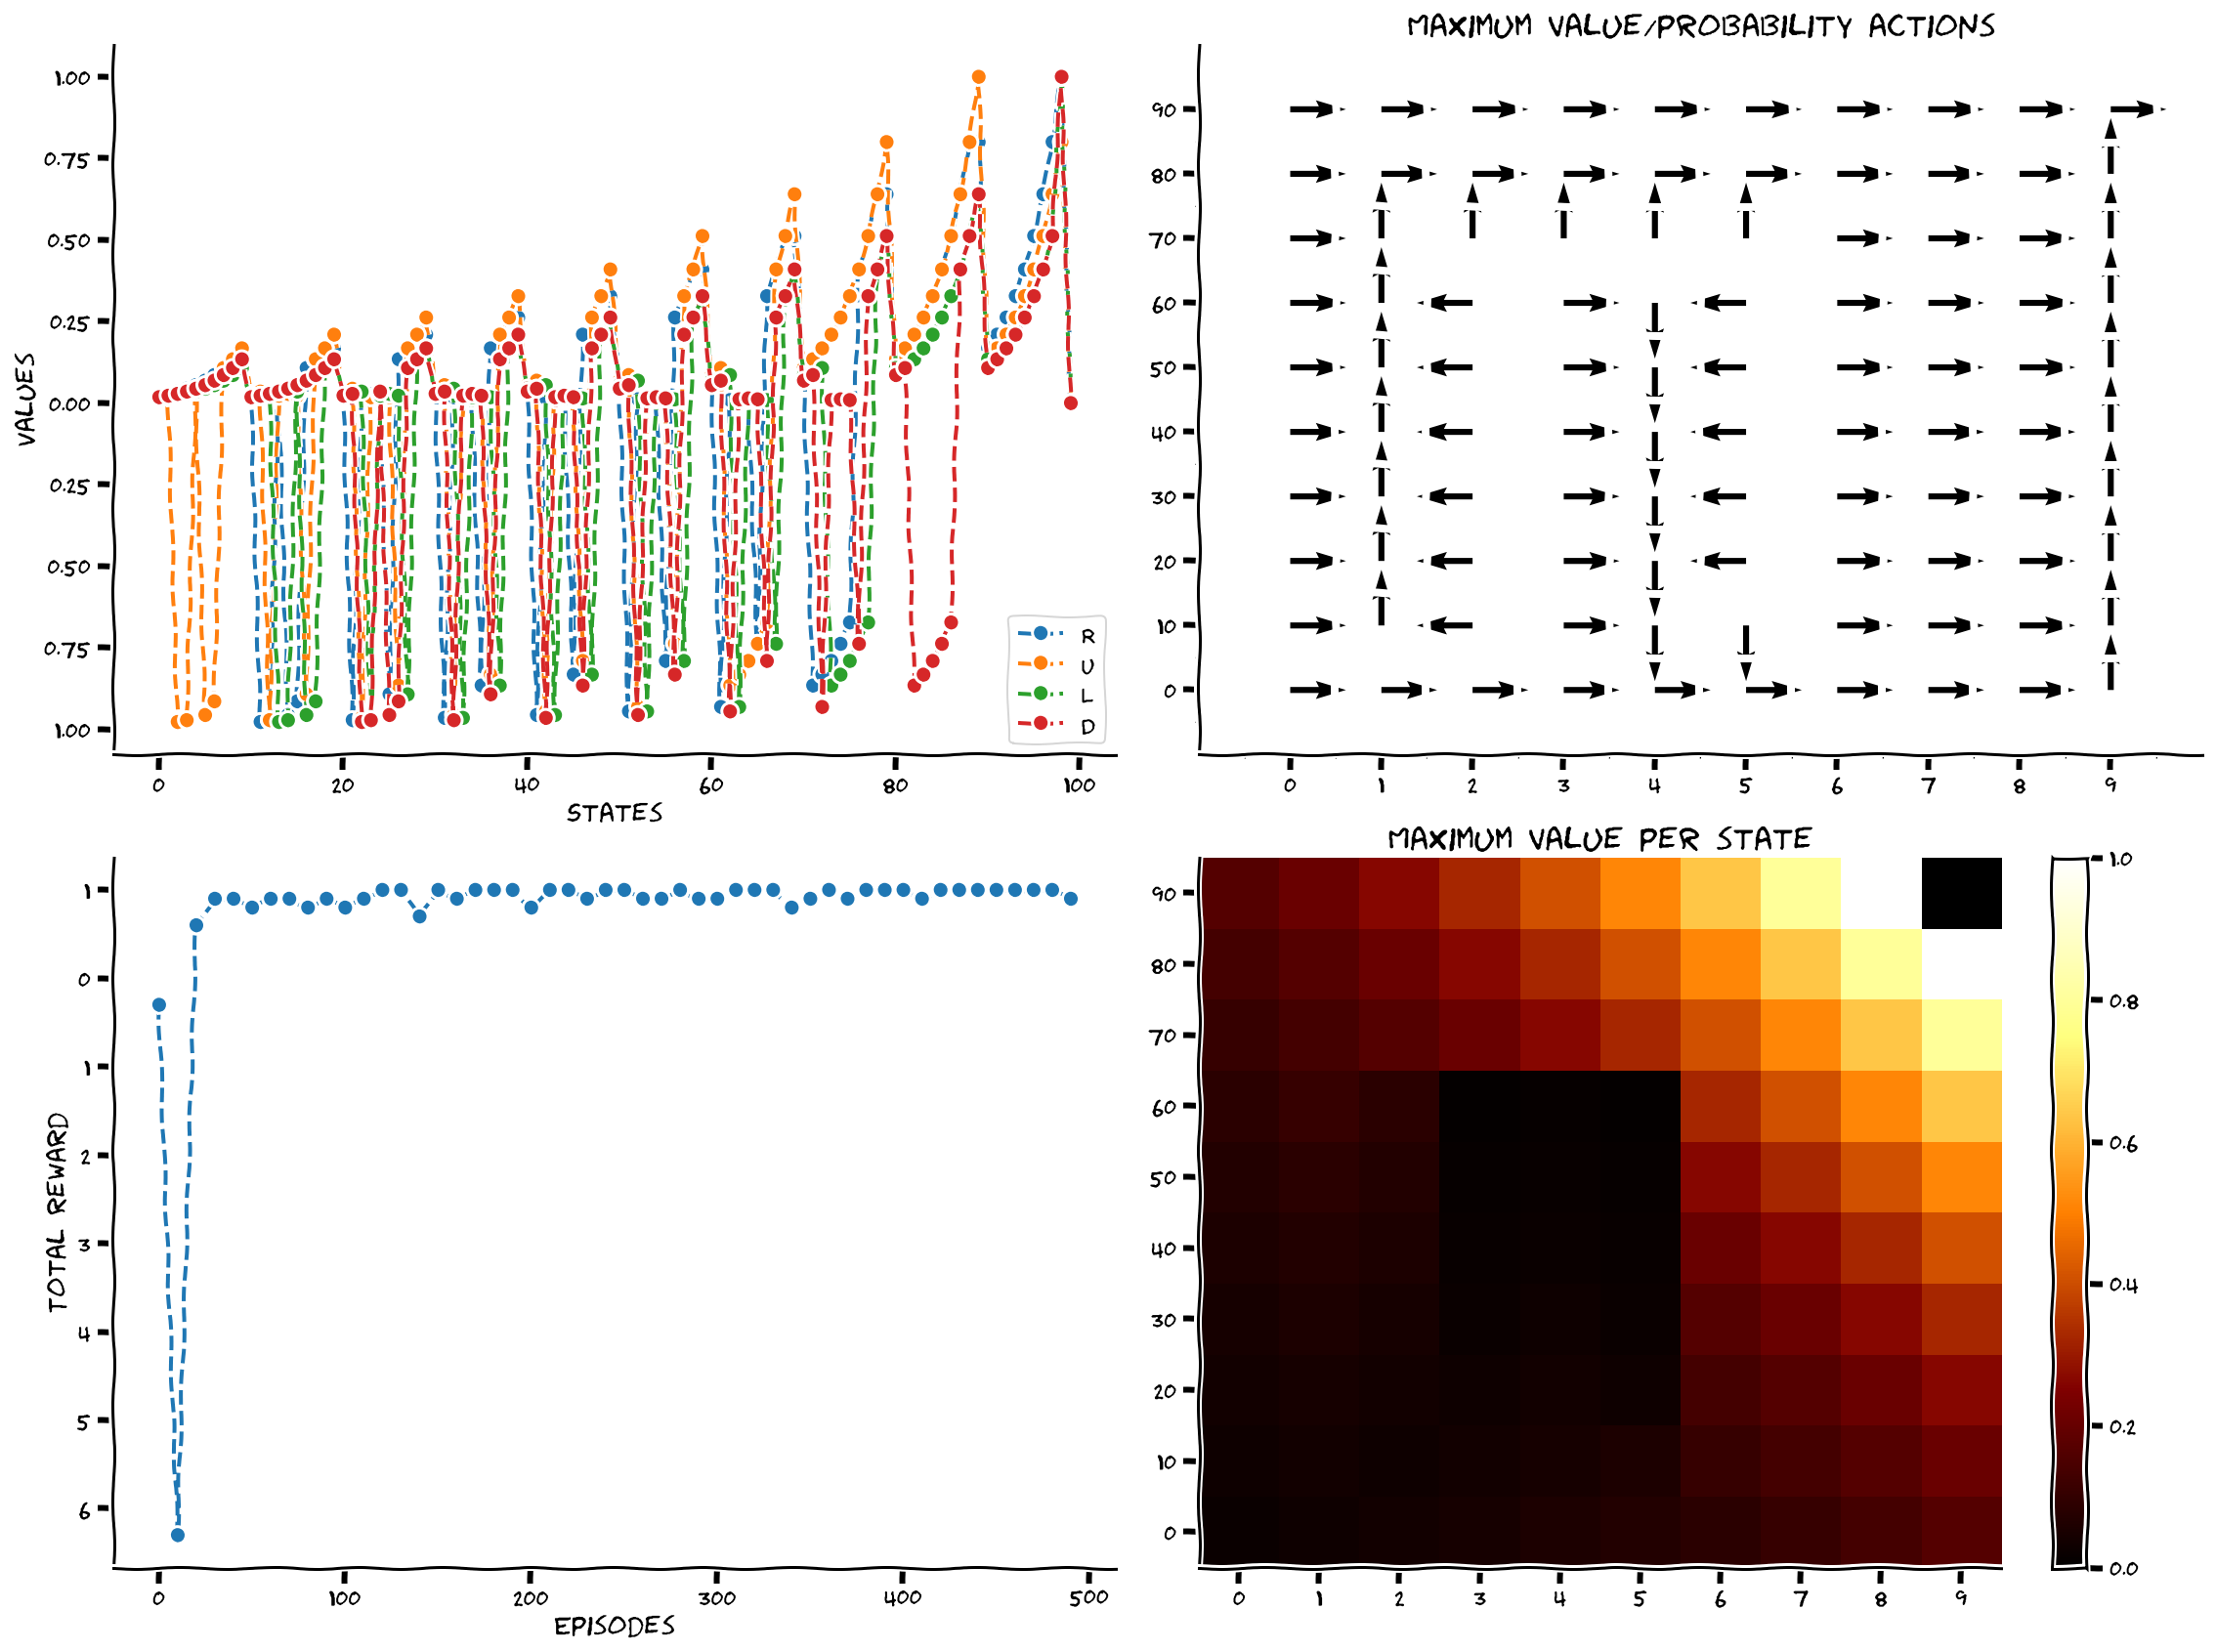
\includegraphics[scale=0.16]{Figures/RL/RL_Figure17.png}
\end{center}

The Dyna-Q agent is able to solve the task quite quickly, achieving a consistent positive reward after only a limited number of episodes (bottom left).

\end{subbox}
\end{textbox}
%%%%%%%%%%%%%%%%%%%%%%%%%%%%%%%%%%%%%%%%%%%%%%%%%%%%%%
%%%%%%%%%%%%%%%%%%%%%%%%%%%%%%%%%%%%%%%%%%%%%%%%%%%%%%
\begin{textbox}{\href{https://compneuro.neuromatch.io/tutorials/W3D4_ReinforcementLearning/student/W3D4_Tutorial4.html}{From Reinforcement Learning to Planning } }

\begin{subbox}{subbox}{How much to plan?}
\scriptsize

We implemented a Dyna-Q agent with $k=10$, we will try to understand the effect of planning on performance. How does changing the value of $k$ impact our agent's ability to learn?

The following code is similar to what we just ran, only this time we run several experiments over several different values of $k$ to see how their average performance compares. In particular, we will choose $k \in \{0, 1, 10, 100\}$. Pay special attention to the case where $k = 0$ which corresponds to no planning. This is, in effect, just regular Q-learning.

The following code will take a bit of time to complete. To speed things up, try lowering the number of experiments or the number of $k$ values to compare.


\begin{center}
    
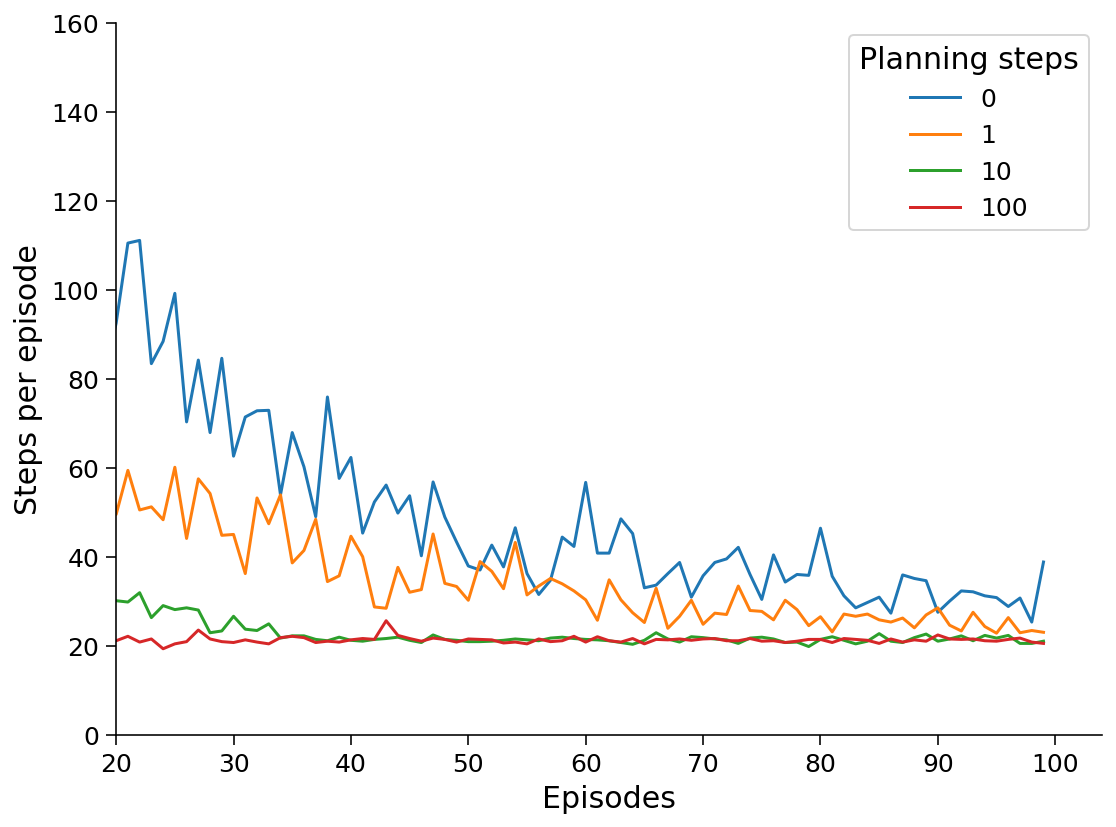
\includegraphics[scale=0.25]{Figures/RL/RL_Figure18.png}
\end{center}
After an initial warm-up phase of the first 20 episodes, we should see that the number of planning steps has a noticeable impact on our agent's ability to rapidly solve the environment. We should also notice that after a certain value of $k$ our relative utility goes down, so it's important to balance a large enough value of $k$ that helps us learn quickly without wasting too much time in planning.

\end{subbox}
\end{textbox}
%%%%%%%%%%%%%%%%%%%%%%%%%%%%%%%%%%%%%%%%%%%%%%%%%%%%%%
%%%%%%%%%%%%%%%%%%%%%%%%%%%%%%%%%%%%%%%%%%%%%%%%%%%%%%
\begin{textbox}{\href{https://compneuro.neuromatch.io/tutorials/W3D4_ReinforcementLearning/student/W3D4_Tutorial4.html}{From Reinforcement Learning to Planning } }
\begin{subbox}{subbox}{When the world changes...}
\scriptsize

In addition to speeding up learning about a new environment, planning can also help the agent to quickly incorporate new information about the environment into its policy. Thus, if the environment changes (e.g. the rules governing the transitions between states, or the rewards associated with each state/action), the agent doesn't need to experience that change *repeatedly* (as would be required in a Q-learning agent) in real experience. Instead, planning allows that change to be incorporated quickly into the agent's policy, without the need to experience the change more than once.

In this final section, we will again have our agents attempt to solve Quentin's World. However, after 200 episodes, a shortcut will appear in the environment.  We will test how a model-free agent using Q-learning and a Dyna-Q agent adapt to this change in the environment.

\begin{center}
    
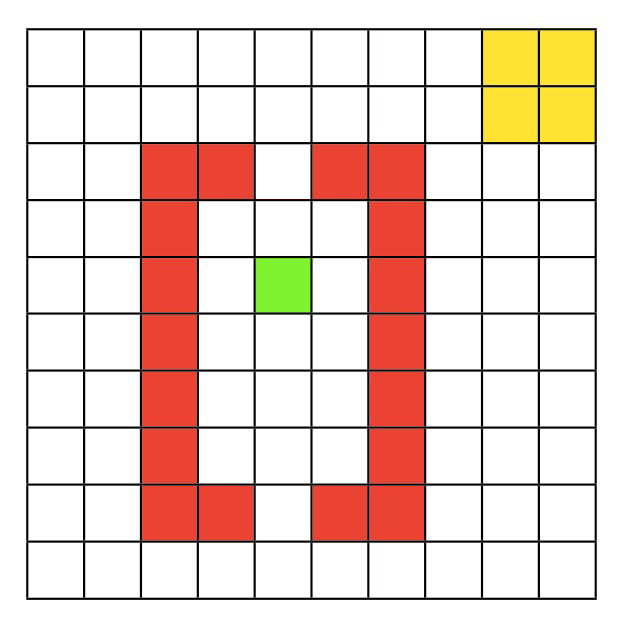
\includegraphics[scale=0.14]{Figures/RL/RL_Figure19.png}
\end{center}
The following code again looks similar to what we've run previously. Just as above we will have multiple values for $k$, with $k=0$ representing our Q-learning agent and $k=10$ for our Dyna-Q agent with 10 planning steps. The main difference is we now add in an indicator as to when the shortcut appears. In particular, we will run the agents for 400 episodes, with the shortcut appearing in the middle after episode #200.

When this shortcut appears we will also let each agent experience this change once i.e. we will evaluate the act of moving upwards when in the state that is below the now-open shortcut. After this single demonstration, the agents will continue on interacting in the environment.
\begin{center}
    
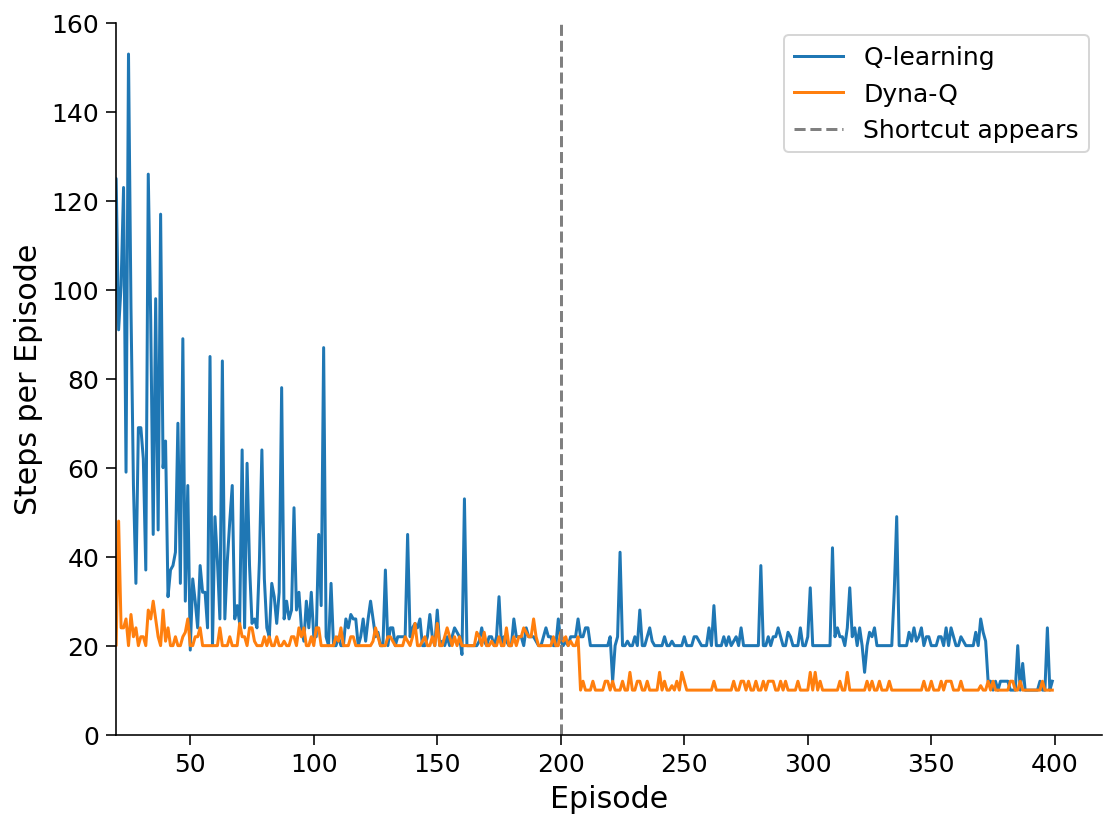
\includegraphics[scale=0.14]{Figures/RL/RL_Figure20.png}
\end{center}

If all went well, we should see the Dyna-Q agent having already achieved near optimal performance before the appearance of the shortcut and then immediately incorporating this new information to further improve. In this case, the Q-learning agent takes much longer to fully incorporate the new shortcut.


\end{subbox}
\end{textbox}
%%%%%%%%%%%%%%%%%%%%%%%%%%%%%%%%%%%%%%%%%%%%%%%%%%%%%%
%%%%%%%%%%%%%%%%%%%%%%%%%%%%%%%%%%%%%%%%%%%%%%%%%%%%%%
\begin{textbox}{\href{https://compneuro.neuromatch.io/tutorials/W3D4_ReinforcementLearning/student/W3D4_Tutorial4.html}{From Reinforcement Learning to Planning } }
\begin{subbox}{subbox}{Summary}
\scriptsize

In this notebook, you have learned about model-based reinforcement learning and implemented one of the simplest architectures of this type, Dyna-Q. Dyna-Q is very much like Q-learning, but instead of learning only from real experience, you also learn from **simulated** experience. This small difference, however, can have huge benefits! Planning *frees* the agent from the limitation of its own environment, and this in turn allows the agent to speed-up learning -- for instance, effectively incorporating environmental changes into one's policy.

Not surprisingly, model-based RL is an active area of research in machine learning. Some of the exciting topics in the frontier of the field involve (i) learning and representing a complex world model (i.e., beyond the tabular and deterministic case above), and (ii) what to simulate -- also known as search control -- (i.e., beyond the random selection of experiences implemented above).

The framework above has also been used in neuroscience to explain various phenomena such as planning, memory sampling, memory consolidation, and even dreaming!

\end{subbox}
\end{textbox}